 \documentclass{article}
\usepackage[utf8]{inputenc}




\usepackage{geometry}                		
\geometry {letterpaper, left=2.5 cm, right=2.5 cm, top=2.5cm, bottom=2.5 cm}    


\usepackage{multirow}
\usepackage{graphicx}		
\graphicspath{ {c:} }
\usepackage{setspace}
\usepackage[version=4]{mhchem}
\doublespace
\usepackage{siunitx}
\usepackage{natbib}
\usepackage{amsmath}
\usepackage{bm}
\usepackage{amsfonts}
\usepackage{lineno}
\usepackage{gensymb}
\usepackage[sharp]{easylist}%makes nice outlines.  Use # for symbol
\usepackage{blkarray}
\usepackage{lastpage}

\begin{document}

%\maketitle

{\Large \noindent \bf %Approaches for handling missing data in ecological time series
Accounting for missing data in autoregressive models of ecological time series
}

\medskip

\noindent Alice Stears\textsuperscript{*}, 
Melissa DeSiervo\textsuperscript{*},
Dusty Gannon,
Amy Patterson,
Alice Carter,
Joanna Blaszczak,
Matt Trentman,
Eliza Grames,
Robert O. Hall, Jr,
Josh Jahner,
Saheed O. Jimoh,
Heili Lowman, % ask Heili again
Courtenay A. Ray,
Christa Torrens,
Lauren Shoemaker$^{\circ}$,
Christopher Weiss-Lehman$^{\circ}$


\noindent Target Journal: Ecology, as a ``Statistical Innovations" article (https://esajournals.onlinelibrary.wiley.com/hub/journal/19399170/author-guidelines) 

\noindent Page count: \pageref{LastPage}/30

\clearpage

%\begin{linenumbers}

\section*{Abstract (198/200 words)} % From Amy's ESA abstract
Long time series are valuable and increasingly available tools for understanding ecological systems. Unfortunately, missing data can impede their utility. While several methods exist, there is no established best practice for handling missing data in autoregressive time series models. Using both simulated data and real time series of primary productivity in a river and great tit population size, we explored the performance of six missing data approaches across scenarios with varying amounts and types of missing data. In each of these scenarios, we assessed how statistical models, fit using each missing data approach, recovered parameters used to simulate data and forecast held out time steps. When data were missing completely at random, regression parameters were recovered well with as many as 50\% missing observations. Conversely, parameter estimates and forecasts were unreliable when data were missing not at random. The best performing missing data approaches were the Kalman filter and data augmentation for time series with Gaussian error (primary productivity example), and data augmentation and complete case data deletion for time series with Poisson error (population size example). Avoid simple data deletion whenever possible, especially for population data, and use extreme caution when data are missing not at random.

\section*{Keywords}
Time series; missing data; autoregressive models

\section*{Introduction} 

Long-term ecological time series contribute to our understanding of many ecological phenomena, from the impacts of species diversity on predator-prey dynamics to patterns of nutrient cycling in ecosystems \citep{Hughes2017, Likens1970, Sinclair2003}. There has been a concerted effort in recent years to facilitate the collection of long-term ecological datasets (e.g. the U.S National Science Foundation Long Term Ecological Research Program (NSF LTER), and the Smithsonian Forest Global Earth Observatory (ForestGEO)), as well as to re-analyze historical long-term datasets with modern methods \citep{Adler2009, Buma2017}. Long-term time series of ecological data, as well as ecological time series in general, are likely to have missing observations, due largely to unpredictable environmental barriers to complete data collection that are difficult if not impossible to overcome \citep{lopucki2022handling, nakagawa_missing_2008}. These include incomplete data collection due to faulty sensors \citep{hossie_confronting_2021}, inaccessibility of field sites due to weather or even a global pandemic, as well as human error during the data entry or collection processes that necessitates removing observations due to inaccuracy. Due to the temporal nature of time series data, it is impossible to retroactively collect data to fill in missing observations. These missing data have cascading negative effects on subsequent analysis including reduced statistical power \citep{kang2013prevention, moritz_imputets_2017} and biased estimation of parameters, leading to both inaccurate and imprecise conclusions \citep{aleryani2018dealing, kim_transcending_2018, junger_imputation_2015}


The prevalence of missing data in ecological time series data is itself problematic, but can be compounded by the characteristics of ecological time series and the statistical approaches used to model them. First, ecological data are often structured as autoregressive time series in which a current data point partially depends on the value of previous data%(e.g., population counts through time or nutrient fluxes within a system)
. This means that each observation is both a response to past observations and a predictor for subsequent observations, so a single missing observation could lead to the effective deletion of multiple data points. %As such, seemingly low rates of missing data in autoregressive time series can have strong negative affects on the precision and bias of statistical inference. 
Further, autoregressive time series with non-Gaussian error distributions are common in ecology, which can add to the challenge of building statistical models and dealing with missing values in these datasets. For example, population count data may be modeled using a Poisson or negative binomial distribution, which precludes the use of classical ARIMA models. Approaches that impute missing values or use model-based approaches that estimate missing values as model parameters must be adjusted to account for time series with non-Gaussian error distributions. 

In addition to accounting for the characteristics of the time series as a whole, one must also account for the missing data mechanism, i.e. the statistical relationship between observations and the probability of missing data. Missing data points can be Missing Completely at Random (MCAR), Missing at Random (MAR), or Missing Not at Random (MNAR) \citep[][Fig. \ref{fig:missingtypes}]{rubin_inference_1976, nakagawa_missing_2015}. Data are MCAR when the probability of a missing observation in the response variable is independent of both the numerical value of observations, as well as the presence or absence of observations in both the response and predictor variables  \citep{nakagawa_missing_2015, horton2007much, newman_missing_2014}. When data are MCAR, the pattern of missingness in the response variable can vary along a spectrum from low autocorrelation (whether a previous time step's data point is missing does not impact whether the current data point is missing) to high autocorrelation (if the previous data point is missing, the current data point is more likely to be missing). Data are MNAR when the probability of missingness in the response variable depends on the numerical value of either the missing observation of the response variable itself (e.g. a temperature sensor can't record values above a threshold, so observations above that value are missing) or an unmeasured predictor variable (e.g.  high streamflows may lead to missing observations in both the stream gage and turbidity sensors, so the missing turbidity values are dependent on the missing stream gage values). Data are MAR when the probability of missingness is not related to the numerical value of the missing observation of the response variable, but is determined by the numerical value of one or more observed predictor variables (e.g. a population age-weight dataset is  missing weights for young-of-the-year because that age class is considered  too delicate to handle ) \citep{newman_missing_2014, ellington_using_2015, nakagawa_missing_2015}. The key difference between MAR and MNAR data is whether the variables that affect missingness are observed (and can thus be conditioned on), which describes MAR data, or unobserved, which describes MNAR data \citep{nakagawa_model_2011}. In addition, once you control for the known variables driving missingness in MAR data, it can be handled like MCAR data \citep{nakagawa_missing_2015}. Our analyses focus on MAR and MNAR only because they are prevalent in ecological time series, and are concerned only with missing values in the response variable, which makes it easier to compare methods across time series with different error structures. Whether data are MAR or MNAR can have a high impact on the accuracy and precision of statistical models and the approaches used to account for missing data \citep{newman_missing_2014, dong2013principled}. 


Fortunately, multiple families of methods exist for dealing with missing data in general (Fig. \ref{fig:ConceptualFigure}). Broadly speaking, these methods can be categorized into simple data processing approaches that occur prior to full statistical analysis or more complex model-based approaches that directly incorporate the missing data into the model-fitting process. The former category primarily consists of data deletion approaches and single imputation \citep{nakagawa_model_2011}. Data deletion is simply removing observations where the data are missing (Fig. \ref{fig:ConceptualFigure} A), while simple imputation `fills in' the missing observation with either the mean, median, or mode of the data, depending on the data type \citep{kang2013prevention, nakagawa_missing_2015, onkelinx_working_2017}. While simple to apply, these methods can be lead to overconfident model precision in the case of single imputation \citep{fichman2003multiple, nakagawa_model_2011, aleryani2018dealing} and reduced statistical power and biased parameter estimates in the case of data deletion \citep{nakagawa_model_2011, aleryani2018dealing}. In contrast to these relatively simplistic methods, several model-based approaches have been developed to directly account for the missing data in the model fitting process. For example, an extension of single imputation, multiple imputation (MI) (Fig. \ref{fig:ConceptualFigure} B), imputes missing data points many times, resulting in multiple new datasets (\textit{m} datasets) where the imputed values vary stochastically for each missing data point, thus allowing uncertainty to be calculated for parameter estimates \citep{rubin1996multiple, rubin1988overview, nakagawa_model_2011, nakagawa_missing_2015}. In contrast to MI, some model-based approaches use iterative algorithms to handle missing data, either by alternating between parameter estimation and data imputation steps (expectation maximization) \citep{nadjafi2022expectation,li2019expectation, kang2013prevention} or by iterating between predicting and updating steps in time series data (Kalman filter) \citep{kalman_filter_1960}. One more recently developed model-based approach, data augmentation (DA), treats the missing data themselves as unknown parameters to be estimated along with the parameters of a specified model for the data-generating process (e.g., means or standard deviations) \citep{kong_sequential_1994}. 

 These approaches for dealing with missing data can and have been applied to ecological data \citep{Newman2023, Soldaat2007}, but we lack a clear sense of how these methods perform relative to one another, particularly when confronted with time series data that have different amounts and types of missing data. Additionally, while the Kalman filter method was developed specifically for autoregressive time series data, it is unclear how the other methods we describe perform when applied to autoregressive time series data. Finally, not all of these methods can be adapted to function with data that do not have a Gaussian error distribution, and when they can be, it is unclear whether using them with Gaussian vs. non-Gaussian distributed data impacts their performance.

Here, we evaluate the precision and accuracy of different statistical approaches for dealing with missing data in autoregressive models of ecological time series data. We test these missing data approaches on real and simulated datasets with both Gaussian and Poisson error distributions. We artificially introduce missingness of different types and increasing amounts into all of these time series, and quantify the performance of different missing data approaches across these three axes of variation in the time series data used (error distribution of the time series, amount of missingness, and type of missingness). This comparison of approaches for dealing with missing data in ecological time series provides a novel comparison of multiple previously-proposed methods of dealing with missing data, some of which have not been previously used with time series. Ultimately, we intend for this comparative study to serve as a resource for ecologists and environmental scientists in search of robust, reproducible methods for confronting time series models with missing data.

\section*{Methods} 

\subsection*{Overview}


Broadly, we compared six approaches for dealing with missing data in time series, and compared their performance when applied to two types of both real and simulated time series with different amounts and types of artificially induced missingness. %Some of these missing data approaches were developed specifically for use in times series, while we adapted others for application to time series data. Additionally, some of these approaches are applied prior to fitting statistical models to a time series, while others are incorporated into the model fitting process. 
In this section, we first discuss the two methods we used to simulate time series with either Gaussian-distributed or Poisson-distributed error. Then, we describe the two empirical* datasets we use, each of which corresponds to one of the simulated data types. *While we recognize that our Gaussian GPP values are modeled using empirical data, for brevity we hereafter refer to both real-world datasets as 'empirical'. We also describe the methods we used to remove observations from both the simulated and empirical time series, which generated time series with different amounts and types of missingness. Finally, we present the six different "missing data approaches" we used to deal with missing observations, and describe how we quantified their relative impacts on the precision and accuracy of statistical models fit to simulated and empirical time series with different amounts and types of missing data.   

\subsection*{Simulated and empirical Gaussian autoregressive time series models}

Time series with Gaussian error distributions and high temporal resolution (which we subsequently refer to as "Gaussian time series") are common in ecology, and are becoming more so as sensors that collect daily or even hourly readings of environmental data become more widely used. In spite of their prevalence, these types of data are prone to missingness \citep{chen2013ecological}. For these reasons, we evaluated the impact of missingness on the efficacy of missing data approaches and the subsequent performance of statistical models using both simulated and empirical data that represent daily measures of environmental and response variables from a sensor. 
%%Overview of our GPP model (mathematical model w/ AR(1), light and discharge%

% To examine parameter recovery across different missingness scenarios in datasets with Gaussian error, we simulated time series data representative of daily measures of environmental and response variables from a sensor. While this type of time series data is increasingly common in ecological studies and produces high-resolution time series, it is prone to data gaps \citep{chen2013ecological}. 
We simulated time series using a first-order auto-regressive (AR(1)) error model with explanatory covariates, such that:

\begin{equation}
    Y_t = {\bf x}_t'{\bm \beta} + \phi (Y_{t-1} - {\bf x}_{t-1}'{\bm \beta}) + \varepsilon_t
\label{eq:ar1}
\end{equation}
where each time step \(Y_t\) is a function of parameters \(\bm \beta\) and matrix transpose of a vector of covariates \({\bf x'}_t\)%, where $'$ denotes the matrix transpose, 
 plus an autoregressive term \(\phi\) times the deviation of the previous time-step from the mean determined by the covariates (i.e. $Y_{t-1} - {\bf x}_{t-1}'{\bm \beta}$). The error term \(\varepsilon_t\) captures both error in this model representation of the variable as well as measurement error, and we assume that $\varepsilon_1, \varepsilon_2,..., \varepsilon_t \overset{iid}{\sim} \mathcal{N}(0, \sigma^2)$ are white noise error terms. For our simulations, we used two covariates and simulated 1000 datasets of 365 observations each, representing a year of continuous sensor data. %We note this example could easily be adapted to any number of covariate relationships and alternative autoregressive structures.

% Explain where the Au Sable datasets come from %%

We fit the above AR(1) model to an empirical dataset of daily river gross primary productivity (GPP) across three years in the Au Sable river in Michigan, USA  \citep{hall_turbidity_2015}. This dataset includes daily GPP (g \(O_2\) \(m^{-2}\) \(d^{-1}\)) (which itself was estimated from measurements of dissolved oxygen, water temperature, and light), as  well as daily measurements of light (\(\mu\)mol \(m^{-2}\) \(s^{-1}\)) and discharge (\(m^{3}\) \(s^{-1}\)). This was the longest, most complete GPP time series we could find, and while it is missing GPP values for 50 days, it still provided 1046 days of data %(we used 699 days for model fitting and 347 days for forecasting). 
In the AR(1) model of this empirical GPP data, we used light and flow as covariates, since they have been identified as primary drivers of GPP \citep{bernhardt_metabolic_2018}. 

\subsection*{Simulated and empirical Poisson population time series model}

Time series with Poisson error distributions (which we subsequently refer to as "Poisson time series"), such as annual counts of population size, are also very common in ecology. Additionally, approaches for dealing with missing data in these types of time series are not as well developed as they are for Gaussian data sets. For these reasons, we evaluated the impact of missing data on model performance using both simulated and empirical data that represent annual counts of individuals in a population. 


We simulated time series data of annual counts of individuals in a population, which have Poisson-distributed error, using a stochastic Ricker population model \citep{ricker1954stock} such that:

%$$
%\begin{aligned}
%\eta_{t+1} &= N_t \cdot e^{r \cdot \left(1 - \frac{N_t}{K}\right)}\\
%N_{t+1} &\sim f(\eta_{t+1})
%\end{aligned}
%$$

\begin{subequations}
\begin{align} \label{eq:ricker2}
    \eta_{t+1} &= N_t e^{(r - \alpha N_t)}\\
    N_{t+1} &\sim f(\eta_{t+1})
\end{align}
\end{subequations}

\noindent where \(\eta_{t+1}\) represents the expected population size at time \(t+1\), \(r\) is the intrinsic, density-independent growth rate of the population, and $\alpha > 0$ is the intraspecific competitive effect that induces negative density dependence. %The population carrying capacity is determined as $K= r/\alpha$. 
Realized population size, $N_{t+1}$, is a random draw from the distribution $f()$ with mean $\eta_{t+1}$. Throughout our simulations, we set $f()$ to be a Poisson distribution with rate parameter $\eta_{t+1}$%, though other error distributions may be appropriate in different empirical applications
. We simulated 1000 datasets of 60 observations each, representing 60 years of annual census data. 

Paralleling our Gaussian model approach, we fit the above Ricker model to a 59-year sequence of annual counts of great tit (\textit{Parus major}) broods in the Wytham woods in Oxford, UK (Ben Sheldon, personal communication, https://wythamtits.com). This census data is continuous from 1960 - 2018. %(we used 48 years for model fitting and 10 years for forecasting).  

\subsection*{Introducing Missingness into Time Series}

To assess the ability of different missing data approaches to account for differing amounts and types of missing data, we created "missing datasets" by systematically removing observations from both the empirical and simulated time series (Fig.\ \ref{fig:missingtypes}). First, we created datasets with data  ``missing completely at random" (MCAR) by removing observations in the response variable using a random process in which the probability of missingness was independent of both the numerical value of the observation and of the covariates. Additionally, the missingness pattern in MCAR data could have high or low autocorrelation, such that missing values were temporally clumped or evenly distributed across the time series. We also created datasets with data ``missing not at random" (MNAR), by removing observations whose numerical value was in the lower or upper tail of the distribution of the response variable. Motivating these two approaches, for a long-term stream sampling dataset, MCAR data might arise due to an individual data logger stopping due to an electronic issue or skipped census dates due to researcher illness, whereas MNAR data might arise due to a flow meter being swept away at high river flows or a temperature logger systematically failing to record observations when the temperature is too low. These scenarios are meant to represent potential missingness-generating processes that would commonly occur in ecological data collection, but are not intended to be exhaustive.

We created MCAR datasets with varying proportions of missing data and degrees of autocorrelation in missingness (Fig.\ \ref{fig:missingtypes}B--E) by viewing a time series as a Markov-modulated Bernoulli process where the variable could have two states: missing or not missing \citep{Gharib2014, Edwards1960}. The probability that an observation in a time series at time \textit{t+1} was missing depended on both the specified proportion of non-missing values in the entire time series ($p$) and the specified degree of autocorrelation in missingness ($\omega$). In a time series $X_1, X_2, ..., X_n$, the transition matrix that describes the probability of an observation at $X_{t+1}$ being missing, based on whether the observation at $X_t$ was missing is defined as: 


\begin{equation}
\begin{blockarray}{rcccc}
\text{} & \BAmulticolumn{4}{c}{X_{t+1}}\\
X_t & \text{Present} & \text{Missing}  \\
\begin{block}{r(cccc)}
\text{Present} & 1-(1-\omega)p & (1-\omega)p \\
\text{Missing} & (1-\omega)(1-p) & \omega + (1-\omega)p  \\
[1ex]
\end{block}
\end{blockarray}
\end{equation}

\noindent We used this transition matrix to stochastically introduce increasing levels of missingness into both empirical and simulated GPP and population count time series. For each unique simulated time series, we created 150 MCAR missing datasets: one for each possible combination of $p$ ranging from 5 to 75\% by increments of 5\% and $\omega$ ranging from 0 to 0.9 by increments of 0.1. We also created 450 MCAR missing datasets using each of the empirical GPP and population count time series, each with a unique combination of $p$ and $\omega$, but in order to more easily examine forecast accuracy across multiple axes of variation, we restricted the possible values of $p$ to 20$\pm$5\%, 40$\pm$5\% and 60$\pm$5\% and the possible values of $\omega$ to 25$\pm$5\%, 50$\pm$5\% and 75$\pm$5\%.

We created Gaussian datasets with data missing not at random (MNAR) by removing observations at both the high and low tails of the distribution of data (Fig.\ \ref{fig:missingtypes}F,G). These types of MNAR scenarios, where the value of the variable itself is related to its probability of missingness, often occur in sensor data similar to our GPP example. However, the MNAR pattern of missingness is unlikely to occur in the population count data with Poisson error because the size of a population in a given year is unlikely to affect the probability of missing data collection that year. (It is important to note that while very low population size may lead to false zeros in a time series of count data, observation error is a problem distinct from missing data). Because of this difference, we did not create MNAR missing datasets for simulated or real data with Poisson error. For each of the simulated AR(1) process time series we created 15 MNAR missing datasets with $p$ increasing from 5 to 75\% by increments of 5\%. To select observations for removal, we first calculated the mean and standard deviation of the time series with no missing data to create a normal distribution, and then identified the threshold values above and below which the density of the normal distribution corresponded to the desired proportion of missingness. We replaced any values above and below those threshold values with an NA. We also created 15 MNAR missing datasets using each the empirical GPP time series, but in order to more easily examine forecast accuracy across multiple axes of variation, we restricted the possible values of $p$ to 20$\pm$5\%, 40$\pm$5\% and 60$\pm$5\%. In total, we generated 
450 MCAR missing datasests with real Gaussian data,
15 MNAR missing datasets with real Gaussian data,
15,000 MNAR missing datasets with simulated Gaussian data,
150,000 MCAR missing datasets with simulated Gaussian data,
450 MCAR missing datasets with real Poisson data, and 
150,000 MCAR missing datasets with simulated Poisson data. 


\subsection*{Comparing missing data approaches}

We evaluated several, previously-published approaches for accounting for missing data: simple and complete data deletion, multiple imputation (MI), the Kalman filter, the expectation maximization (EM) algorithm, and Bayesian data augmentation (DA) (Fig.\ \ref{fig:ConceptualFigure}; see below for more detailed descriptions). We used four of the methods for both Gaussian and Poisson data types, but only used the Kalman filter for Gaussian data, and only used expectation maximization for Poisson data. %We fit either an AR(1) (for Guassian data) or Ricker (for Poisson data) statistical model to each of the simulated and empirical time series. 
In the cases of both types of data deletion and multiple imputation, we applied the missing data approach \textit{before} fitting the corresponding statistical model. For the simulated and empirical population count time series, we fit a Poisson generalized linear model (GLM) with the \texttt{glm} function from the \texttt{stats} package in R \citep{r_2021}. For the simulated and empirical GPP data, we fit an AR(1) model with two covariates using the \texttt{arima} function from the \texttt{stats} package in R \citep{r_2021}. For the Kalman filter, expectation maximization, and data augmentation approaches, the missing data were addressed simultaneously with the model fitting process (Fig. \ref{fig:ConceptualFigure}). We describe the methods we used to implement each of these missing data approaches in the sections below that describe each approach.  

\noindent\textbf{Impact of missing data and missing data approach on parameter recovery:} We used models fit to \textit{simulated} time series to determine how the missing data approach, data type (i.e. Gaussian or Poisson data), and the type and amount of missingness affected a model's ability to recover the model parameters used to simulate the data. For both types of simulated time series, applied a missing data approach and fit a statistical model to the full extent of the time series. We then compared the model-derived parameter estimates to the parameters used in each simulation. The parameters we evaluated were $\phi$ and the $\beta$ coefficients for each covariate from the AR(1) models, and $\alpha$ and $r$ for the Ricker models.

We then compared measures of bias and precision of parameter recovery by models fit to data with a given data type, missingness type (MNAR or MCAR with low, medium, or high autocorrelation), amount of missing data and missing data approach. First, we calculated relative error,$e_s = \frac{\hat{\theta}_s - \theta_s}{\theta_s}$, and absolute relative error, $|e_s| = \frac{\hat{\theta}_s - \theta_s}{|\theta_s|}$ for each parameter in each model, where $e_s$ is the relative (or absolute relative) error of $\hat \theta_s$, which estimates the true parameter $\theta_s$ for simulation $s$. These relativized values allowed us to compare parameter recovery across datasets with different simulation parameters as well as compare different parameters in a given model (e.g, regression coefficients to auto-regressive coefficients). A relative error of 0 indicates perfect parameter recovery for that simulation, while a positive or negative error indicates an over or under estimate of a parameter, respectively. Then, we grouped models first by Gaussian or Poisson data type, then by the missing data approach used (data deletion, multiple imputation, etc.), the type of missingness in the time series used to fit the model (MCAR or MNAR), and proportion of missingness (rounded to the nearest 10\%). Finally, we categorized MCAR datasets as ``low autocorrelation" ($25 \pm 5\%$), ``moderate autocorrelation" ($50 \pm 5\%$), and ``high autocorrelation" ($75 \pm 5\%$).

Within each of these `bins' of models, we calculated the median of the relative error ( which we call "Median error"), median absolute relative error ("Median absolute error"), and interval coverage for each model parameter ("Coverage"). We used the median of the relative error distribution as an estimate of bias due to heavy tails in the error distribution and finite simulation numbers. A positive or negative median error indicates systematic over- or under-estimation of that parameter in a given model bin, respectively. The median absolute error gives an idea of the variance of the estimator. A high median absolute relative error indicates that an approach leads to unstable estimates across models fit to many simulated datasets. Coverage indicates the proportion of times in a bin when the 95\% confidence interval from a fitted model contains the true parameter. A coverage value closer to 0.95 indicates that an approach comes with appropriate measures of uncertainty. We note that, since the two $\beta$ parameters in the AR(1) model of Gaussian data were simulated using the same data generating process, we pooled their estimates together. We ultimately used these metrics of the central tendency (median relative error) and spread (median absolute relative error) of the error distribution, as well as coverage to understand how the missing data approach and the amount and type of missingness impacted parameter recovery in models fit to simulated time series with Gaussian or Poisson error.

\noindent\textbf{Impact of missing data and missing data approach on forecast accuracy:} 
We used models fit to empirical time series to determine the impact of missing data approach, data type, and the type and amount of missingness on a model's ability to forecast held-out data. For both types of empirical time series we fit statistical models to a portion of the times series, and then used the resulting model to forecast the remaining time steps. In the Au Sable GPP time series, models were fit to the first two years of daily GPP data (~66\% of the total time series), and then the resulting model parameters were used to forecast the remaining year of daily GPP (~33\%) (Fig. \ref{fig:ParamRec_Gauss} A). In the great tit population size time series, we used the first 49 years of brood size counts (83\%) to fit models, and then used the resulting model parameters to forecast the last 10 years of data (17\%).

We then compared model forecasts to the observed values for the forecasted part of each time series, and calculated the root mean square error (RMSE) of each forecast. As described above, we then binned these RMSE values according to the type of data used to fit the model (GPP or population data, MAR or MNAR missingness, $p$, and $\omega$), and then by the missing data approach used. This RMSE value indicated the accuracy with which a model was able to forecast future time steps, with higher RMSE values indicating lower precision and accuracy, and lower RMSE values indicating higher precision and accuracy.     


\subsection*{Missing Data Approaches}

\noindent\textbf{Simple and Complete Data deletion:} 
% State what we did [what pkg did we use for the data deletion? We used nothing special, at least for the Ricker sims we simply did the deletion using standard methods and then used glm from base R stats to fit the model] 
We considered two different data deletion methods in our analyses. The ``simple data deletion" approach involves removing missing values from a time series, compressing the dataset, and running the model as if the time intervals between observations were all equal (Fig. \ref{fig:ConceptualFigure} A). This method violates the assumption of equal temporal spacing between observations -- an assumption implicit in most time series models -- but we include it here as a reference because it simple and commonly used in published studies. We also include ``complete case data deletion," which is a slightly more rigorous approach than simple data deletion but is still easy to implement. This approach maintains equal spacing between observations by removing a missing value itself as well as the subsequent observation(s) that is predicted by the missing value (Fig. \ref{fig:ConceptualFigure} A). However, those observations after a missing value are retained as predictors of the subsequent observation(s). 


\noindent\textbf{Multiple imputation: }Multiple imputation (MI) is an approach for addressing problems of missing data that systematically fills in missing observations with imputed values, and creates several different versions of complete data sets that can be used to estimate uncertainty around each imputed value (Fig. \ref{fig:ConceptualFigure} B). MI is commonly used in ecology, with multiple studies evaluating methods and approaches to conduct MI for functional traits \citep{taugourdeau_filling_2014,johnson_handling_2021,penone_imputation_2014}, population biology \citep{onkelinx_working_2017}, time series \citep{hui_gap-filling_2004}, and meta-analyses \citep{ellington_using_2015}.  MI’s effectiveness can depend on the number of imputed datasets (\textit{m}). It is often assumed that \textit{m}=5 is a minimum value \citep{honaker_what_2010}; however, researchers have used \textit{m}=200 when comparing methods in the ecological sciences \citep{onkelinx_working_2017}. In general, larger values of \textit{m} result in more accurate estimates of both parameter values and uncertainty. %However, increasing \textit{m} results in a trade-off between accuracy and computation time; this can be particularly problematic for data-rich (e.g., long time series) or complex (e.g., hierarchical) models. 
After imputing the \textit{m} data sets, the analyses of interest are confronted with each data set, and the estimated parameters from the \textit{m} analyses are averaged using Rubin rules of averaging to get the parameter(s), and associated uncertainty, from which inference can be made. We implemented multiple imputation with the Amelia II package in R \citep{honaker2011}, which uses an expectation maximization algorithm (see below) in combination with a bootstrapping technique for deciding what values to impute. We used $m=5$ in order to provide decent estimates without excessive run times.

For both the simulated and empirical population count time series, since we did not have any covariates, the only variables used for imputation were the population size at time \textit{t} and population size at time \textit{t-1}. For time series with chunks of missing data, the Amelia multiple imputation function had to be run iteratively, with missing values filled in from the edges of the missing chunks. In addition, while the recommended settings for dealing with time series data using the Amelia package include incorporating preceding and proceeding time points by specifying the ``lags" and ``leads" options \citep{honaker2011}, it was not possible to use the lags option, since the current population was already using the population at the previous point as its only predictor for imputation. Instead, we included only the leads option, which still resulted in occasional failure of the method at extremely high levels ($>70\%$) of missing data due to excessive collinearity between the preceding and proceeding time points. The lack of error handling for extremely collinear variables is an unfortunate issue for this method when using data sets without covariates, or data sets with highly collinear covariates.  

For both the simulated and empirical Gaussian series, implementing multiple imputation was more straightforward since an observation at time \textit{t} was informed by two covariates in addition to the observation at the time \textit{t-1}. In this case, we were able to use both the ``lags" and ``leads" options in \texttt{amelia}. 

Following execution of multiple imputation using Amelia II, we fit statistical models to time series following the methods described in \textbf{Comparing missing data approaches}. 

\noindent\textbf{Kalman Filter:} The Kalman Filter was developed to estimate the state of a dynamic system that is observed with error but can be used to derive the likelihood function of a time series with missing observations (Fig. \ref{fig:ConceptualFigure} C). To illustrate the approach, assume a state-space model

\begin{equation*}
    \begin{aligned}
        X_t &= \phi X_{t-1} + \epsilon_t \\Y_t &= X_t + e_t
    \end{aligned}
\end{equation*}
where $X_t$ is the true ``state" of the system at time $t$, $Y_t$ is the observed value at time $t$, and $\epsilon_t \sim \mathcal{N}(0, \sigma^2)$ and $e_t \sim \mathcal{N}(0, \tau^2)$ are IID white noise error terms for the process and observation error, respectively. The Kalman Filter is primarily focused on estimating the unobserved state of the system, $X_t$, and can be conceptualized as a two-step procedure in which, given an initial state $X_0$, we can forecast the next state $X_1$. Then, following data collection at the next time point, $y_1$, we update the forecast using Bayes' theorem. Specifically, the forecast distribution for $X_1$ is
\begin{equation*}
    p(x_1) = \int p(x_1 | x_0)p(x_0)dx_0
\end{equation*}
where $p(\cdot)$ denotes the probability density function. Assuming IID Gaussian errors, $p(x_1)$ is normal with mean ${\tilde x}_1 = \phi x_0$ and variance $v_1 = \phi^2 \frac{\sigma^2}{1 - \phi^2} + \sigma^2$. Given the observed value $y_1$, we update the estimate of $X_1$ using Bayes theorem
\begin{equation*}
    \begin{aligned}
        p(x_1 | y_1) &\propto p(y_1 | x_1) p(x_1)
        &= \mathcal{N}\Bigl(\tilde x_1 + K_1(y_1 - \tilde x_1),\ (1 - K_1)v_1 \Bigr)
    \end{aligned} 
\end{equation*}
where $K_1 = v_1 / (v_1 + \tau^2)$ is the \textit{Kalman gain} and creates a weighted average of the forecast and observation. %If the observation error is large, the forecast is favored as an estimate of $X_t$, whereas if the process noise is large relative to the observation error, the estimate of $X_t$ tends towards the observed value $y_t$.
For our focus on missing data, we assume the process is observed without error such that $Y_t = X_t$ and $\tau^2 = 0$. Without observation error, the Kalman gain $K_t = 1$ for all $t$ since $\tau^2 = 0$, and $p(x_1 | y_1) = \mathcal{N}(y_t, 0)$. Thus, the update step gives complete information about $X_t$, and the likelihood function can be defined based on the data $y_1,...,y_n$. However, if data are missing, the update step cannot occur. So, in the case of missing data without observation error, the Kalman Filter alternates between pure forecast steps when data are missing and pure ``update" steps when data and the state of the system are completely observed, but the forecast steps yield a method for computing the likelihood function recursively without needing to know the states of $X_t$ in which we were unable to observe the process and therefore have no associated $y_t$.


The Kalman filter assumes a Gaussian error distribution, so we only used this method with the simulated and empirical Gaussian time series. We implemented the Kalman filter missing data approach at the same time as the model fitting process, where we fit an AR(1) model with two covariates using the \texttt{arima} function from the \texttt{stats} package in R \citep{r_2021} (the Kalman filter is the default algorithm used to handle missing values in this R function). 

\noindent\textbf{Expectation maximization algorithm: }The expectation maximization (EM) algorithm is an iterative algorithm that is conceptually similar the Kalman Filter, and recursively computes the likelihood of a time series with missing data (Fig. \ref{fig:ConceptualFigure} D). Given an initial guess for the parameter vector we wish to estimate, ${\bm \theta}_0$, the first step (Expectation step) proceeds to ``fill in" the missing observations with their expectation given the observed data and the initial parameter vector ${\bm \theta}_0$ %. For example, if $Y_t$ were missing, we impute $Y_t$ with $\mathbb{E}(Y_t | y_{t-1}, {\bm \theta}_0)$
, which is equivalent to the forecast step of the Kalman filter conditioned on ${\bm \theta}_0$. In the second step (maximization step), we compute the maximum likelihood estimate of ${\bm \theta}$ using the filled-in time series as data to give an updated estimate $\hat {\bm \theta}_1$. We then iterate this process, updating the forecasts of the missing data using their expectations conditional on $\hat {\bm \theta}_1$, then maximizing the likelihood with respect to $\bm \theta$ using the time series filled-in with the updated forecasts. This process is iterated until the difference between successive estimates is acceptably small, indicating convergence (that is, $||\hat {\bm \theta}_i - \hat {\bm \theta}_{i-1}||_1 < \delta$ for some small $\delta > 0$).

Given its similarity to the Kalman filter, we only used this missing data approach for the simulated and empirical Poisson time series. We constructed an approximate EM algorithm to estimate the parameters of the Ricker model in which missing data were rounded to the nearest integer value during the expectation step such that the likelihood was well-defined for the filled-in series. As such, the missing data were dealt with at the same time as the model fitting process. We used the \texttt{optim} function from the \texttt{stats} package in \texttt{R} for the maximization step \citep{r_2021}. In Figure S1%\ref{fig:EM-bias-checks}
, we show that the estimates are asymptotically unbiased. Note that the algorithms required to estimate standard error of parameter estimates generated from EM are notoriously unstable and difficult to implement in R, so the results of models we fit using this missing data approach do not include standard error estimates. 


\noindent \textbf{Data augmentation: }Data augmentation (DA) provides a model-based framework for estimating missing observations as well as the parameters of interest, but comes with the added benefit of standard errors for the estimates of all the unknown quantities by treating the missing observations as additional parameters to be estimated (Fig. \ref{fig:ConceptualFigure} D). We fit the Gaussian AR(1) models with DA and Stan \citep{carpenter_stan_2017} by using the rstan \citep{rstan_package} and brms \citep{burkner2017brms} packages in R \citep{r_2021}. Data augmentation for the population model is not possible with Stan, however, due to the requirement of continuous parameter space for the Hamiltonian Monte Carlo (HMC) methods Stan uses to sample the posterior distribution (at least not without marginalizing out the discrete parameters, which proved intractable). Treating missing integer data as parameters was therefore not possible with Stan, and partially-known parameter vectors are not supported in JAGS. We therefore designed a Gibbs sampler with Metropolis updates for the log growth factor ($r$) and intra-specific competition coefficient ($\alpha$), and Gibbs sampling of any missing observations, $N_{t}^{(0)}$, conditional on $(r, \alpha, {\bf N}_{t-})$, where ${\bf N}_{t-}$ is the vector of abundances (both observed and unobserved) up to but not including time $t$. We used weakly informative Gaussian priors for $r$ and $\ln(\alpha)$ and fit the models using custom functions written in R. %Figure \ref{fig:bias-checks} shows that this algorithm also converges on the ``true" parameter values with increasing sample sizes. 



%\begin{enumerate}
 %   \item Comparing the performance of model approaches for simulated data 
%\begin{enumerate}
 %   \item compare the accuracy of parameter recovery for different methods -- are estimates biased? 
 %   \item compare the precision of different approaches (i.e. average SD for each parameter estimate or 95\% CI across all simulations for each parameter estimate) 
  %  * Q: do we want to do this for all parameters? For just a couple?-- maybe combine fixed effects of light and discharge somehow? 
   % * potentially include the rate at which models fail? (i.e. how sharply does the rate of model non-convergence increase as the amount of missingness increases?)
%\end{enumerate}
%\item Comparing the performance of model approaches for real data 
%\begin{enumerate}
%    \item compare of methods in terms of estimation error (compare forecast RMSE)
%\end{enumerate}
%\end{enumerate}

%* Explain how we did this uniquely for Gaussian and Poisson error, for models using MNAR data with increasing amounts of missingness and then for models using MAR data with both increasing levels of missingness and autocorrelation

\section*{Results}

\subsection*{Parameter recovery in Gaussian models}

For the Gaussian MCAR simulated data, all approaches had similarly accurate and precise $\beta$ parameter estimates across all levels of missing data, with median error and median absolute error below 10\% and confidence interval coverage very near 95\%. In contrast, estimates of the $\phi$ parameter were more affected by missing data, and some missing data approaches performed better than others (Fig. \ref{fig:ParamRec_Gauss}). Notably, the data augmentation and Kalman filter methods had the strongest overall performance, with low error and high coverage of $\phi$ estimates with as much as 60\% missing data. All other methods lost both accuracy and CI coverage as the amount of missing data increased. The two data deletion methods, simple and complete-case, had essentially the same ability to recover $\phi$. Both of these methods had increasing median error and absolute median error as the amount of missingness increased, while coverage dropped as low as $\sim70\%$ (see Fig. \ref{fig:ParamRec_Gauss}). The multiple imputation method had the worst performance of all five Gaussian approaches across every level of missing data. Coverage dropped sharply when more than 10\% of the data were missing, while median and median absolute error steadily increased with any amount of missing data. In some cases, multiple imputation would underestimate the parameter value by over 50\%. The combination of high error and low CI coverage seen in the lowest-performing missing data approaches demonstrate that they could be especially misleading, with a high probability of generating incorrect estimates of the autocorrelation parameter ($phi$, in this case) with incorrectly low  uncertainty. 

Misleading parameter estimates are an even greater concern when fitting models to Gaussian MNAR data.  Whereas inaccurate and overly precise estimates are really only an issue with the $phi$ parameter in models fit to Gaussian MCAR data, our analysis indicate that with MNAR data, these misleading estimates would occur for both $\beta$ and $\phi$ parameters, with every missing data approach, and at every level of missing data (Fig. \ref{fig:ParamRec_Gauss}). With MNAR data, all missing data approaches tended to underestimate $\phi$ by up to 95\%, and overestimate $\beta$ by up to $\sim40\%$.  CI coverage plummeted from $\sim75\%$ with low missing data, to below 50\% when 10\% of the data were missing, and ended close to 0\% coverage with 40\% or more of the data missing (see Fig. \ref{fig:ParamRec_Gauss}). 


%\subsubsection*{Autocorrelation in missingness}
The degree of autocorrelation in missing data also affected parameter recovery, but only for data deletion methods and only for $\phi$ (see Fig. SX for the effect of autocorrelation on $\beta$ estimates). Specifically, higher levels of autocorrelation led to more accurate estimates of $\phi$ when either complete case or simple data deletion were used (Fig. \ref{fig:heatMap_gauss_MAR}). This is most likely because higher levels of autocorrelation in missingness preserved longer segments of intact data, which are important for estimating autoregressive parameters such as $\phi$. However, it is important to note that our simulations assumed no change in parameter values through time (i.e. generated stationary time series), so long stretches of intact data are equally valuable in the model fitting process regardless of when they occur in the time series. If this assumption were violated, high autocorrelation in missingness might not have the same beneficial effect on parameter estimates.   

\subsection*{Parameter recovery in Poisson models}
When fitting Ricker models to simulated, Poisson distributed MCAR time series, the simple data deletion missing data approach recovered both r and $\alpha$ model parameters substantially worse than other methods, particularly as amounts of missing data increased (Fig. \ref{fig:ParamRec_Pois}). Among the remaining methods, expectation maximization consistently had low median error and absolute median error. Interestingly, complete-case data-deletion also had low median error, similar to expectation maximization, but higher median absolute error than EM; however, this pattern was reversed for data augmentation, which recovered parameters with relatively higher median error than EM, but lower median absolute error. Finally, multiple imputation recovered parameters with higher values of both median error and median absolute error, though was still much more accurate and precise when compared to simple data deletion. These trends were very similar for estimates of both $r$ and $\alpha$, reflecting the fact that estimates of growth and competition parameters are correlated in Ricker-type models \citep{bender1984perturbation}. Similar to the results for Gaussian time series, autocorrelation in missing data lead to more accurate parameter estimates for the simple data deletion method, but had little impact on other methods (Fig. SX).

When considering the coverage of parameter estimates from each method, several important patterns arise. First, simple data deletion had the lowest coverage among all methods (Fig. \ref{fig:ParamRec_Pois}). Taken together with its poor performance in terms of error, this suggests that methods relying on simple data deletion will be particularly dangerous as parameter estimates are likely to be quite inaccurate but accompanied by overly narrow confidence intervals. Just as in the Gaussian simulations, this same problem applies to multiple imputation, though to a lesser extent than for simple data deletion. On the other hand, data augmentation and complete-case data deletion both maintain close to 95\% coverage across a range of missing data amounts, suggesting these methods are accurately quantifying uncertainty around parameter estimates. Importantly, expectation maximization does not provide standard error for parameter estimates so coverage for this method cannot be assessed. Researchers should therefore only consider expectation maximization if they do not need to account for uncertainty in parameter estimates.


\subsection*{Forecasting and missing data}
Introducing different levels of missing data in an empirical time series with a Gaussian error distribution revealed several important implications for forecasting accuracy. First, when data are missing completely at random (MCAR), both the median and variance of forecast Root Mean Squared Error (RMSE) across many model runs increased with higher amounts of missing data (Fig. \ref{fig:RMSE_Gaus} B). This effect was strongest for the variance of RMSE. Thus, while in this case it is possible to generate relatively accurate predictions with high levels of missing data, the likelihood of accurate predictions from any given model fit to high missingness data is largely dependent on which individual data points are missing. Second, all missing data approaches perform similarly in terms of forecast RMSE. This could be a reflection of the relative importance of the environmental parameters in the model as these were much less impacted by missing data compared to the autocorrelation ($\phi$) parameter (Fig. \ref{fig:ParamRec_Gauss}). Finally, and similarly to the results for parameter recovery, when data were missing not at random (MNAR), model forecasts had substantially increased RMSE as the amount of missingness increased. In fact, only 20\% of data MNAR led to worse forecasts across methods than when 60\% of the data were MCAR. Variance of RMSE did not meaningfully change as the amount of data MNAR increased. 

As with the Gaussian time series, both the median and variance of forecast RMSE increased as the amount of missing data increased in an empirical time series of population counts (Fig. \ref{fig:RMSE_Poiss}). This pattern was consistent across all of the missing data approaches we evaluated. In particular, the variance of forecast RMSE increased substantially as missingness increased, underscoring that the specific  data points missing in a time series can strongly affect the accuracy of model fit and predictions. While most methods performed similarly in these forecasts, multiple imputation had generally lower lower median RMSE, particularly at higher amounts of missing data. It should be noted, though, that RMSE is relatively high across all methods and amounts of missing data. 

\section*{Discussion}

 Missing data is a nearly ubiquitous phenomenon in ecological studies and can be particularly problematic when fitting autoregressive time series models, since missing values violate the key statistical assumption of observations that are equally spaced in time. We evaluated six previously proposed methods for dealing with missing data by fitting autoregressive models to simulated and empirical examples of two different types of time series common in ecology: daily observations of a continuous variable with a Gaussian error distribution (analogous to sensor data) and annual observations of a discrete variable with a Poisson error distribution (analogous to count data, such as trends in population size). 
 
Our results indicate that parameter estimation can be fairly robust to missing data, as long as the error distribution of the time series, the type of missingness (MCAR vs MNAR), and amount of auotocorrelation in missingness are taken into account: thus missing values in time series do not necessarily have a catastrophic effect on model accuracy, precision, or forecast ability. In fact, several methods, such as data augmentation and the Kalman filter when applied to Gaussian data and expectation maximization when applied to Poisson data could recover simulation parameters with relatively high accuracy and precision even when 50\% of observations were missing completely at random (although we do not suggest fitting models to time series with this much missing data). Similarly good performance was found for high missingness in non-time series data \citep{graham_missing_2009}. While we found several missing data approaches that performed well for a range of data and missingness types, we also identified some approaches that were uniformly unsuitable. Simple data deletion, where observations that are missing are simply deleted from the time series, led to inaccurate and imprecise models despite being one of the commonly used methods in ecological analyses. Multiple imputation was also quite inaccurate and imprecise, especially for fitting AR(1) %ARIMA 
models to data with a Gaussian error distribution. Additionally, we found that when data are missing not at random (MNAR), none of the methods we considered here provided robust parameter estimates. Handling non-random missingness requires some knowledge about the missingness mechanism such that the likelihood of missingness can itself be modeled, which is often a tall order in ecological systems  \citep[e.g.,][]{Sotto2011_mnar, McCall2014_mnar, Shoari2018_mnar} Below, we further explore the impacts of the different amounts and types of missing data we considered on model performance, and provide more specific recommendations for missing data approaches given certain types of data and missingness.

First, it is essential to identify the mechanism of missingness in the data, i.e. the structure behind the missing data values, because it informs selection of the best missingness approach. If the values are MCAR in a time series, our results provide a first-pass guide to identifying suitable missing data approaches. Within each data type, each of the missing data approaches we evaluated tended to perform consistently well or poorly in terms of parameter recovery (Fig. \ref{fig:ParamRec_Gauss}, Fig. \ref{fig:ParamRec_Pois}) The best-suited approach will depend on research goals and characteristics of the time series itself, but include more recommendations below about methods that should be avoided or performed consistently well with MCAR data. Conversely, the missing data approaches we assessed provide universally poor parameter recovery and forecast accuracy for time series with MNAR data. We therefore do not recommend any of the missing data approaches we evaluated when missing values are MNAR, i.e. whether an observation is missing depends on the variable itself or on a 'missing' value of some unmeasured/ unaccounted-for variable. %[ADDRESS HOW TO ID MISSING DATA.] 
This is consequential, since it is likely that many ecological timeseries contain data that are MNAR \citep{bowler2025treating}. Because MNAR missingness depends on unobserved values, it can be inferred but is difficult to prove (\citep{nakagawa_missing_2015}). However, if the variables or processes behind MNAR missingess can be identified, observed, and controlled for in the modeling process, the missing data can be treated as missing completely at random, which then makes common missing data approaches more viable \citep{newman_missing_2014, nakagawa_missing_2015}. Therefore, it is important for researchers to carefully consider their study system, identify drivers that could potentially lead directly or indirectly to data that are MNAR, and then ensure they measure these drivers. It is also useful to record reasons for missing observations when they occur, in order to develop an understanding of the mechanism driving missingness in a system. In short, MNAR data can have dire consequences for precision and accuracy, but thoughtful investigation and planning prior to time series collection can mitigate the negative impacts.  

While our analyses indicate that the most suitable missing data approach will depend on many factors, we can make some general recommendations. First, choice of missing data approach should be informed by the goal of an analysis, and what sort of information is necessary for further analytical steps. For example, if you require numerical estimates of missing values, then out of the approaches we evaluated, only multiple imputation and data augmentation would suit your needs. An additional general recommendation is that, regardless of the data type, amount and type of missingness, or the analysis goal, simple data deletion should be used only with the utmost caution--advice that has been emphasized previously \citep[e.g.,][]{nakagawa_model_2011, Shoari2018_mnar,lopucki2022handling}. Simple data deletion has the tendency to substantially over or underestimate parameter estimates and underestimate confidence intervals of those parameters. This effect was considerable in the case of models we fit to Poisson distributed simulated data (Fig.\ \ref{fig:ParamRec_Pois}), but was less extreme in parameters from models fit to simulated Gaussian data (Fig.\ \ref{fig:ParamRec_Gauss}). This may be due to the fact that the AR(1) model we used for Gaussian data included two covariates that did not have missing values, while the Ricker model we used for Poisson data did not have covariates. %Interestingly, simple data deletion led to the widest range of forecast RMSE when forecasting the great tit empirical dataset with 60\% missing data (Fig.\ \ref{fig:RMSE_Poiss}B), suggesting that the predictive performance of this approach is inherently tied to the composition of the missing data. This complexity was also found in the empirical Gaussian forecasting, where simple data deletion was the best for missing not at random and among the worst for missing at random treatments (Fig.\ \ref{fig:RMSE_Gaus}B). Inconsistency in predictive performance across datasets is troubling, and makes the use of simple data deletion even more questionable. 
While it may be intuitive that simply removing data points creates irregular time-steps and violates model assumptions, simple data deletion is straightforward to implement and can actually occur under the hood in some modeling packages without being obvious to the user. For example, many R functions include arguments for automatically removing NA values (e.g. na.exclude, na.omit, na.rm, etc.), which are easy to utilize without an adequate understanding of their implications. Fortunately, there are several other missing data approaches we examined here that are straightforward to implement, are more robust that simple data deletion, and don't violate underlying assumptions of time series models.

%(Could this also serve as a call to develop methods streamlining other ways to deal with missingness?). 
%For example, the \texttt{arima()} function from package \texttt{stats} requires the presence of \texttt{NA} values in place of the missing data (rather than dropping \texttt{NA}'s from the data) in order to properly account for unequal spacing among observed values. 


For Gaussian time series with missingness completely at random (MCAR), every missing data approach we evaluated was able to recover the parameters for $\beta$ covariates with consistently high coverage and low error (Fig. \ref{fig:ParamRec_Gauss}). If you have Gaussian data and care more about the covariate ($\beta$s) than autoregressive ($phi$) parameters, any of the missing data approaches could work for you, although we still recommend avoiding simple data deletion because it violates a key model assumption. If you also prioritize accurate and precise autoregressive parameter ($\phi$) recovery, your options are more limited if you have more than ~10\% of observations MCAR. Only two approaches had similarly strong recovery of $\phi$: the Kalman filter and data augmentation. These methods also remained effective at every level of autocorrelation in missingness (Fig. \ref{fig:heatMap_gauss_MAR}). In contrast, both of the data deletion methods (simple and complete case) had consistently poor performance for $\phi$ recovery, although their median error at a given level of missingness was reduced when autocorrelation in missingness was higher; while we hope you have already ruled out using simple data deletion, complete case data deletion may be a decent and simple to implement option if missingness is autocorrelated. Multiple imputation was not the worst method but it was far from the best, so we would not recommend it for autoregressive parameter estimation, despite being a commonly recommended method for ecologists \citep{nakagawa_missing_2008,ellington_using_2015}.  When forecasting with the Gaussian data, all approaches performed well, with an RMSE $<$ 1 even at relatively high levels of missing data (Fig. \ref{fig:RMSE_Gaus} B). We believe this is largely because the environmental covariates are much more important for forecasting the mean response than is the autoregressive parameter. Thus, because all approaches had strong covariate parameter recovery, they were all able to forecast well.

 We found that several missing data approaches performed differently when we applied them to Poisson time series with data MCAR. Parameter recovery was more uniform across all of the approaches than with Gaussian data, but complete case data deletion, expectation maximization, and data augmentation were the most accurate and precise for parameter recovery (Fig \ref{fig:ParamRec_Pois}). %Also, with the Poisson data, increasing autocorrelation was only a factor for simple data deletion rather than both simple and complete case data deletion as occurred with the Gaussian data (Fig S_). 
We hypothesize that the difference in the performance of missing data approaches between Gaussian and Poisson time series were due to the difference in model structure between the Ricker model and AR(1) model: The Ricker model only uses abundance at the previous time step,  $t – 1$, to predict abundances at time $t$. In contrast, the AR(1) uses both the value of the response at $t-1$ as well as two covariates to predict a value at time $t$. The relatively simple structure of the Ricker model we used may explain why complete case data deletion performed well with Poisson data but poorly with Gaussian data. %, and was not affected by autocorrelation in missingness.
Forecasts using models fit to Poisson MCAR time series had high RMSE values across all missing data approaches (Fig. \ref{fig:RMSE_Poiss}, which is likely because we relied solely on density-dependence in the Ricker model to capture variation in this time series, and did not include other covariates. However, previous analyses of the great tit dataset we used have suggested that such simplistic models, even if they incorporate environmental drivers, may be inadequate to describe fluctuations in this dataset, and that more complex functional relationships or spatial processes may be necessary \citep{lebreton1990modelling}. Regardless of the overall high RMSE, median forecast error increased markedly as the amount of missing data increased for all missing data approaches, especially when compared to the amount that RMSE increased in forecasts of Gaussian data (Fig. \ref{fig:RMSE_Gaus} B). This indicates that missing data can be particularly damaging to forecasts that use autoregressive models with no covariates. 
         
% P5 -  Topher's "caveats" paragraph? Contains info from 3/12 minutes as well as info added ... a while ago. - CT
Our results provide important insights into the performance of a variety of methods for dealing with missing data in ecological time series, however, we note that our simulations should perhaps best be viewed as benchmarks demonstrating best and worst case scenarios. For example, we did not explore all the nuances of each available method due to computational constraints, but several of the methods could be `tuned' to achieve better of worse performance (e.g., MI might perform better if using more imputed datasets \citep{honaker_what_2010} while the Kalman Filter might perform worse when setting the Kalman gain below one to account for observation error \citep{kalman_filter_1960}). Further, we chose to only explore the effect of missing data in the response variable, and assumed no missingness in the covariates. However, ecological datasets can often have missing data in the covariates as well as the response, which would likely reduce model performance compared to our results. Similarly, we chose an empirical dataset of stream GPP with known, strong effects from environmental covariates \citep{hall_turbidity_2015,bernhardt_metabolic_2018}, meaning the accurate estimates of $beta$ parameters likely played a large role in achieving accurate forecasts even in scenarios where the autoregressive parameter estimates were estimated poorly. In more exploratory scenarios or systems with weaker covariate effects, inaccurate estimates of autoregressive parameters might have larger, negative effects on model forecasting ability. Finally, we only explored scenarios with data Missing Completely At Random and data Missing Not at Random (MCAR and MNAR), representing opposite ends of a spectrum from best to worst case scenarios \citep{newman_missing_2014}. While we did not explore scenarios with data Missing At Random (i.e., with the probability of missingness dependent on one or more covariates; \citep{newman_missing_2014}), we argue model performance in this case would fall in between our two MCAR and MNAR scenarios. Since MAR data would be more likely to be missing for certain values of environmental covariates, the parameter estimates associated with those covariates would likely suffer \citep{nakagawa_missing_2008} with cascading effects for the model's predictive accuracy. How closely the results for such a MAR scenario would fall to the two scenarios we present would depend on the strength of the relationship between covariate values and the probability of missingness and which values of the covariate were most likely to cause missingness. For example, missingness associated with one or both of the extremes of the covariate would be more likely to cause bias in estimates of the associated $\beta$ parameter than missingness associated with average values of the covariate (assuming a linear relationship between the covariate and the response variable). 

Collectively, our comparison of missing data approaches provide a starting guide for dealing with missing data in ecological time series. Our results, especially for the AR(1) model fit to time series with Gaussian error, suggest that parameter estimation and forecast accuracy can be robust to relatively high MCAR missingness -- especially if using the "best" method for accounting for missingness -- this is unlikely to hold for all data types or model structures. This is especially true for shorter time series. As a result, we suggest that running similar simulations to those shown here with data that specifically mirror the length, error distribution, and missingness pattern of your own would data be extremely beneficial when deciding how to best deal with missing observations; we argue that this step should become part of the analysis workflow, particularly in a field-based discipline such as ecology where missing observations are often unavoidable. %For ecologists wanting to apply these date missingness data approaches, we suggest simulating data according to the model(s) they will use and missingness type of their data, to compare methods and better understand systematic bias and uncertainty when working with data with missing values. 



%\end{linenumbers}

\newpage


\section*{Figures}

%% Figure 1

\begin{figure}[!htb]
     \noindent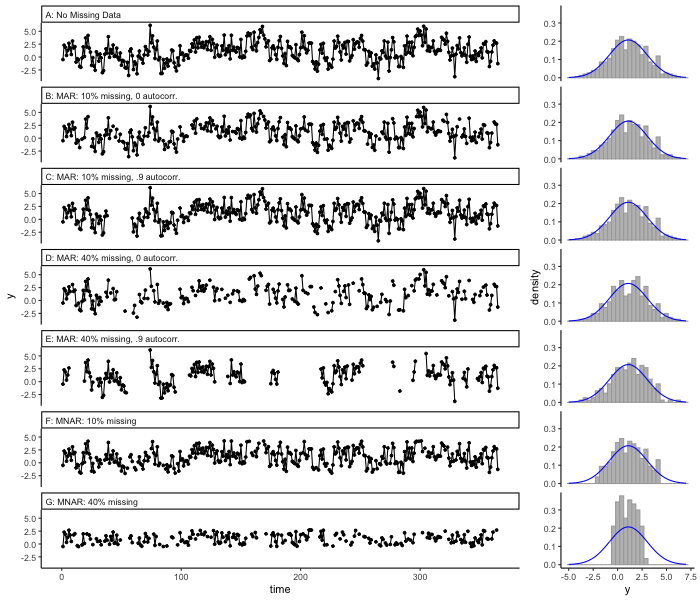
\includegraphics[width = 0.85\textwidth]{Figures/CompareMissingnessTypes_fig.png}
     \caption{An example time series demonstrating different types and amounts of missing data. The left column shows the same time series with different amounts and types of missingness and right column shows the distribution of data points in each resultant time series. A. Complete time series with no missing data. Rows B through E show the time series with 10\% (B and C) or 40\% (D and E) of data missing completely at random (MCAR), with either low autocorrelation in missing data (B and D) or high autocorrelation (C and E). Rows F and G show the time series with data missing not at random (MNAR) for 10\% missing data (F) and 40\% missing data (G).}

     \label{fig:missingtypes}
 \end{figure}



%% Figure 2
\begin{figure}[h]
     \noindent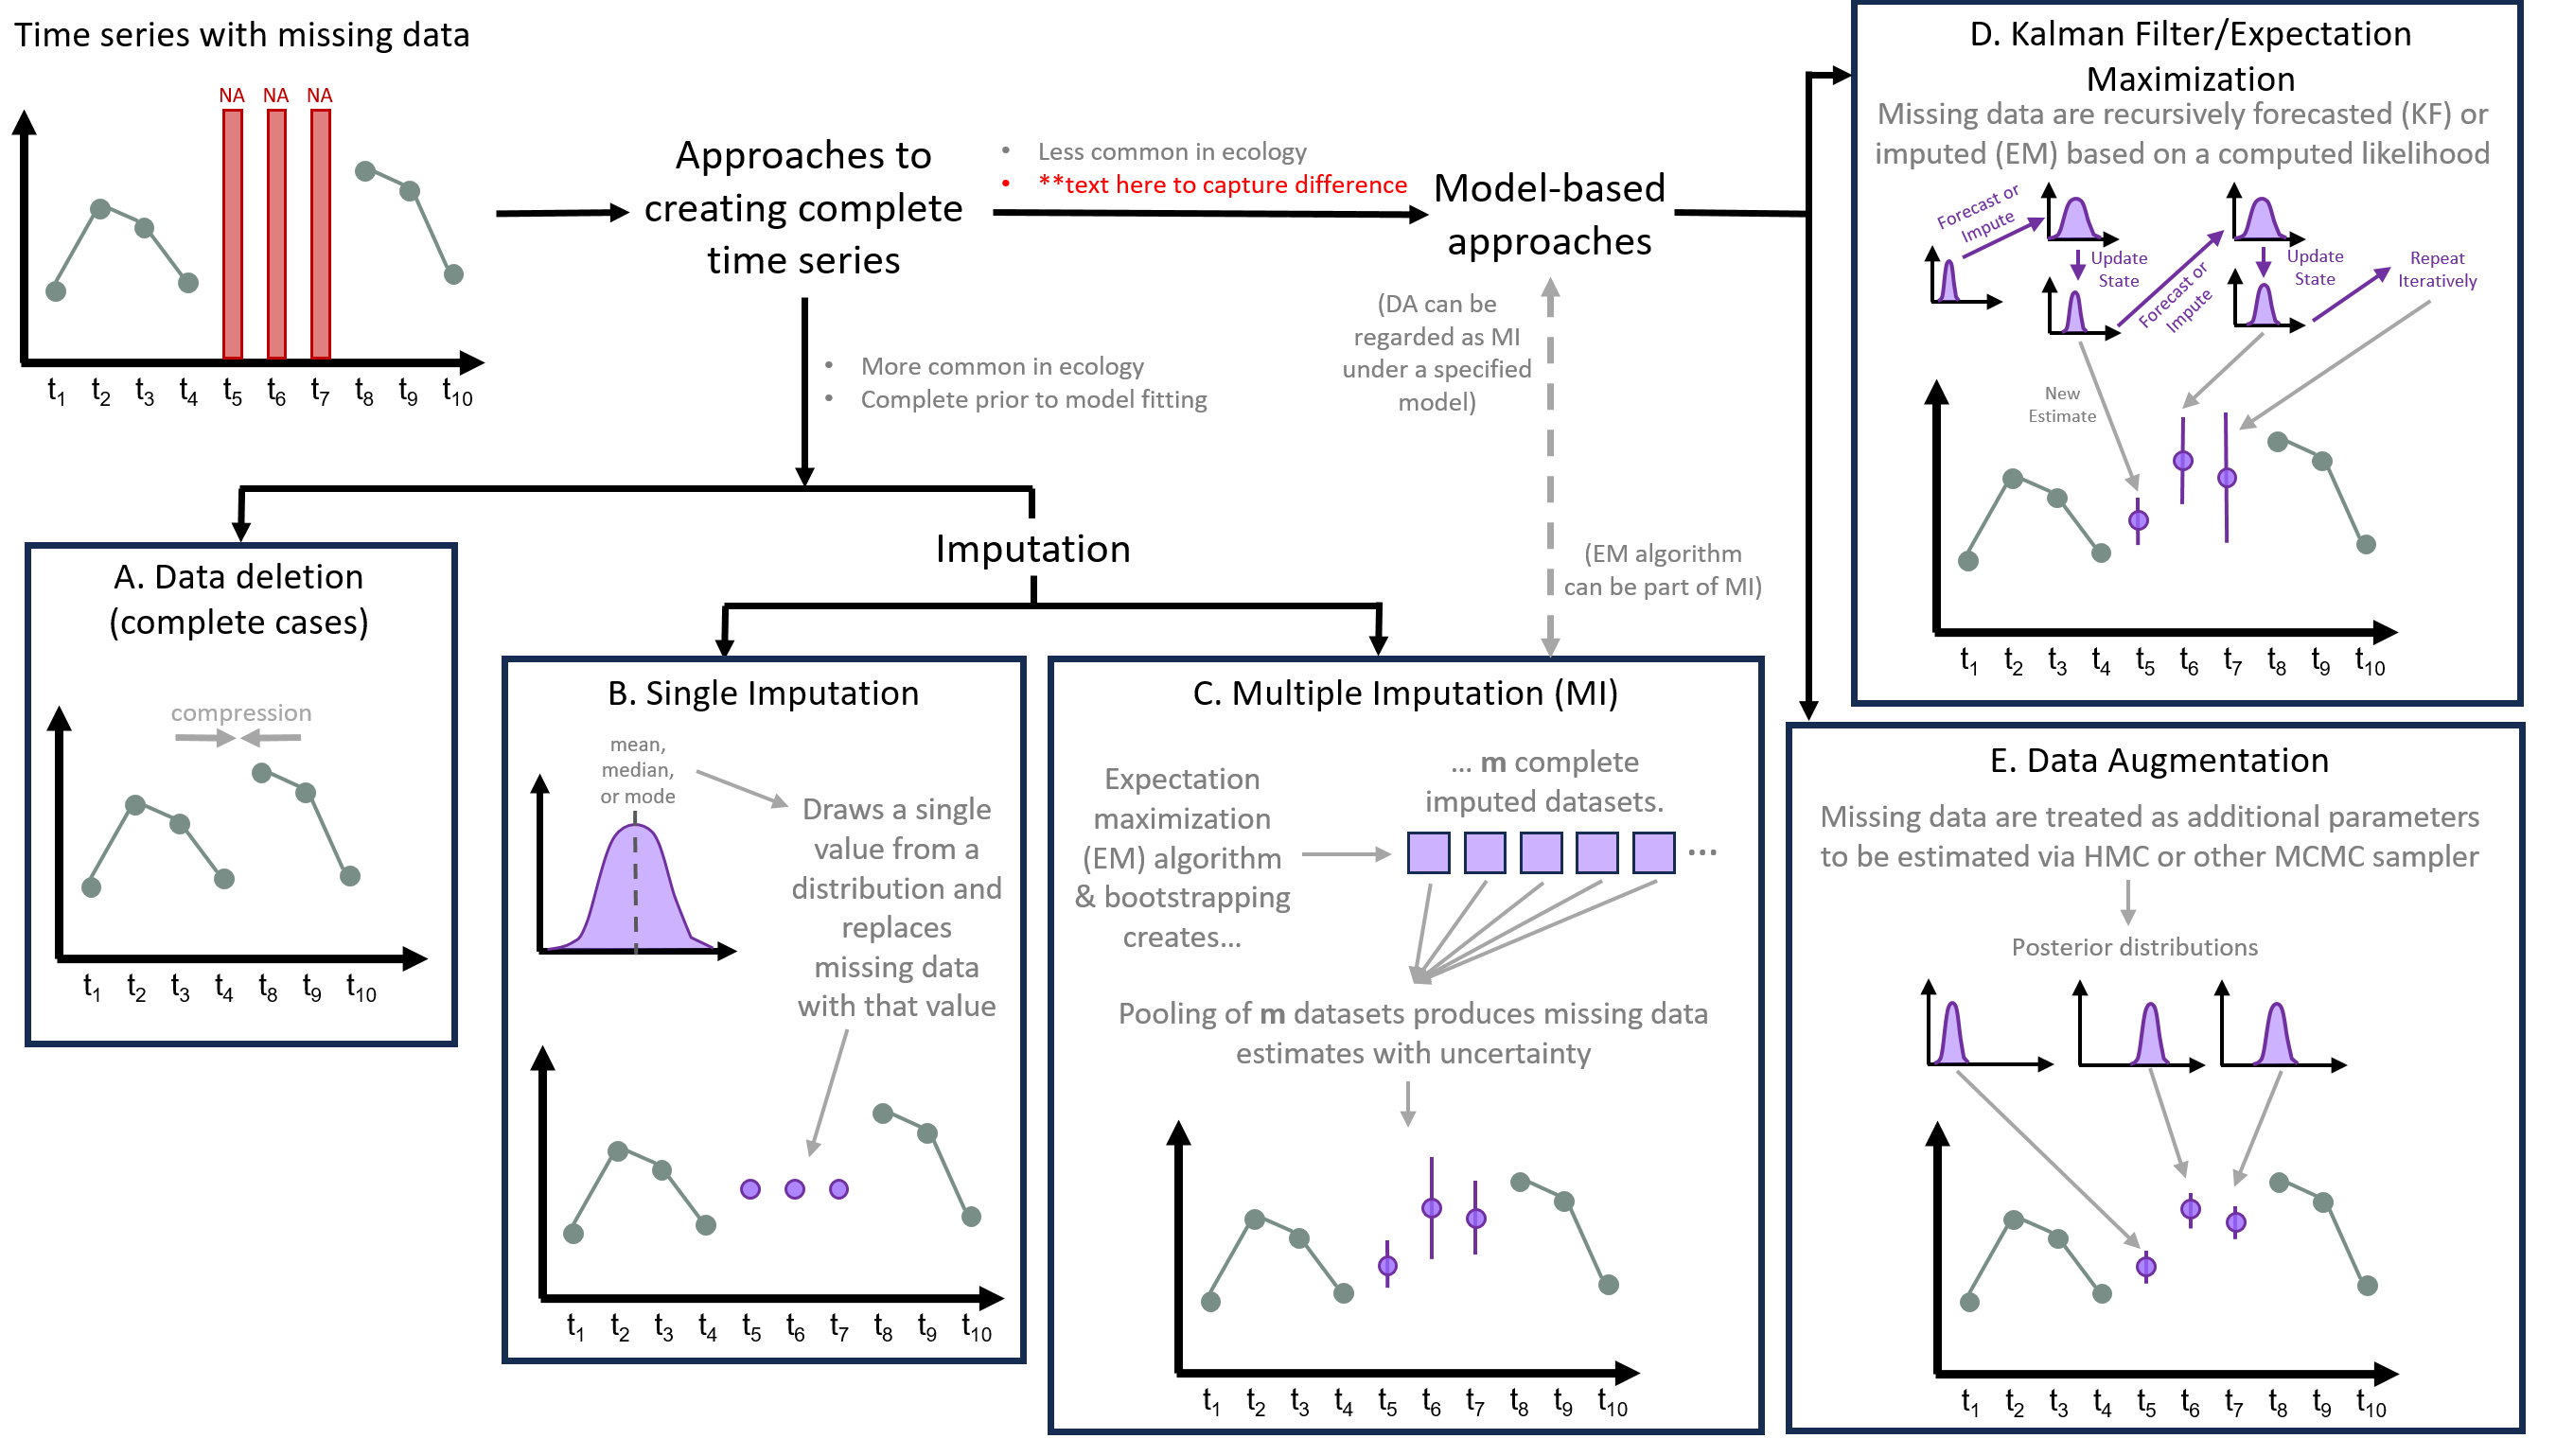
\includegraphics[width = 0.9\textwidth]{Figures/ConceptualFigure.png}
     \caption{Conceptual figure showing different approaches to handling missing data and the mechanisms for each approach}
     \label{fig:ConceptualFigure}
 \end{figure}

%% Figure 3
\begin{figure}
    \noindent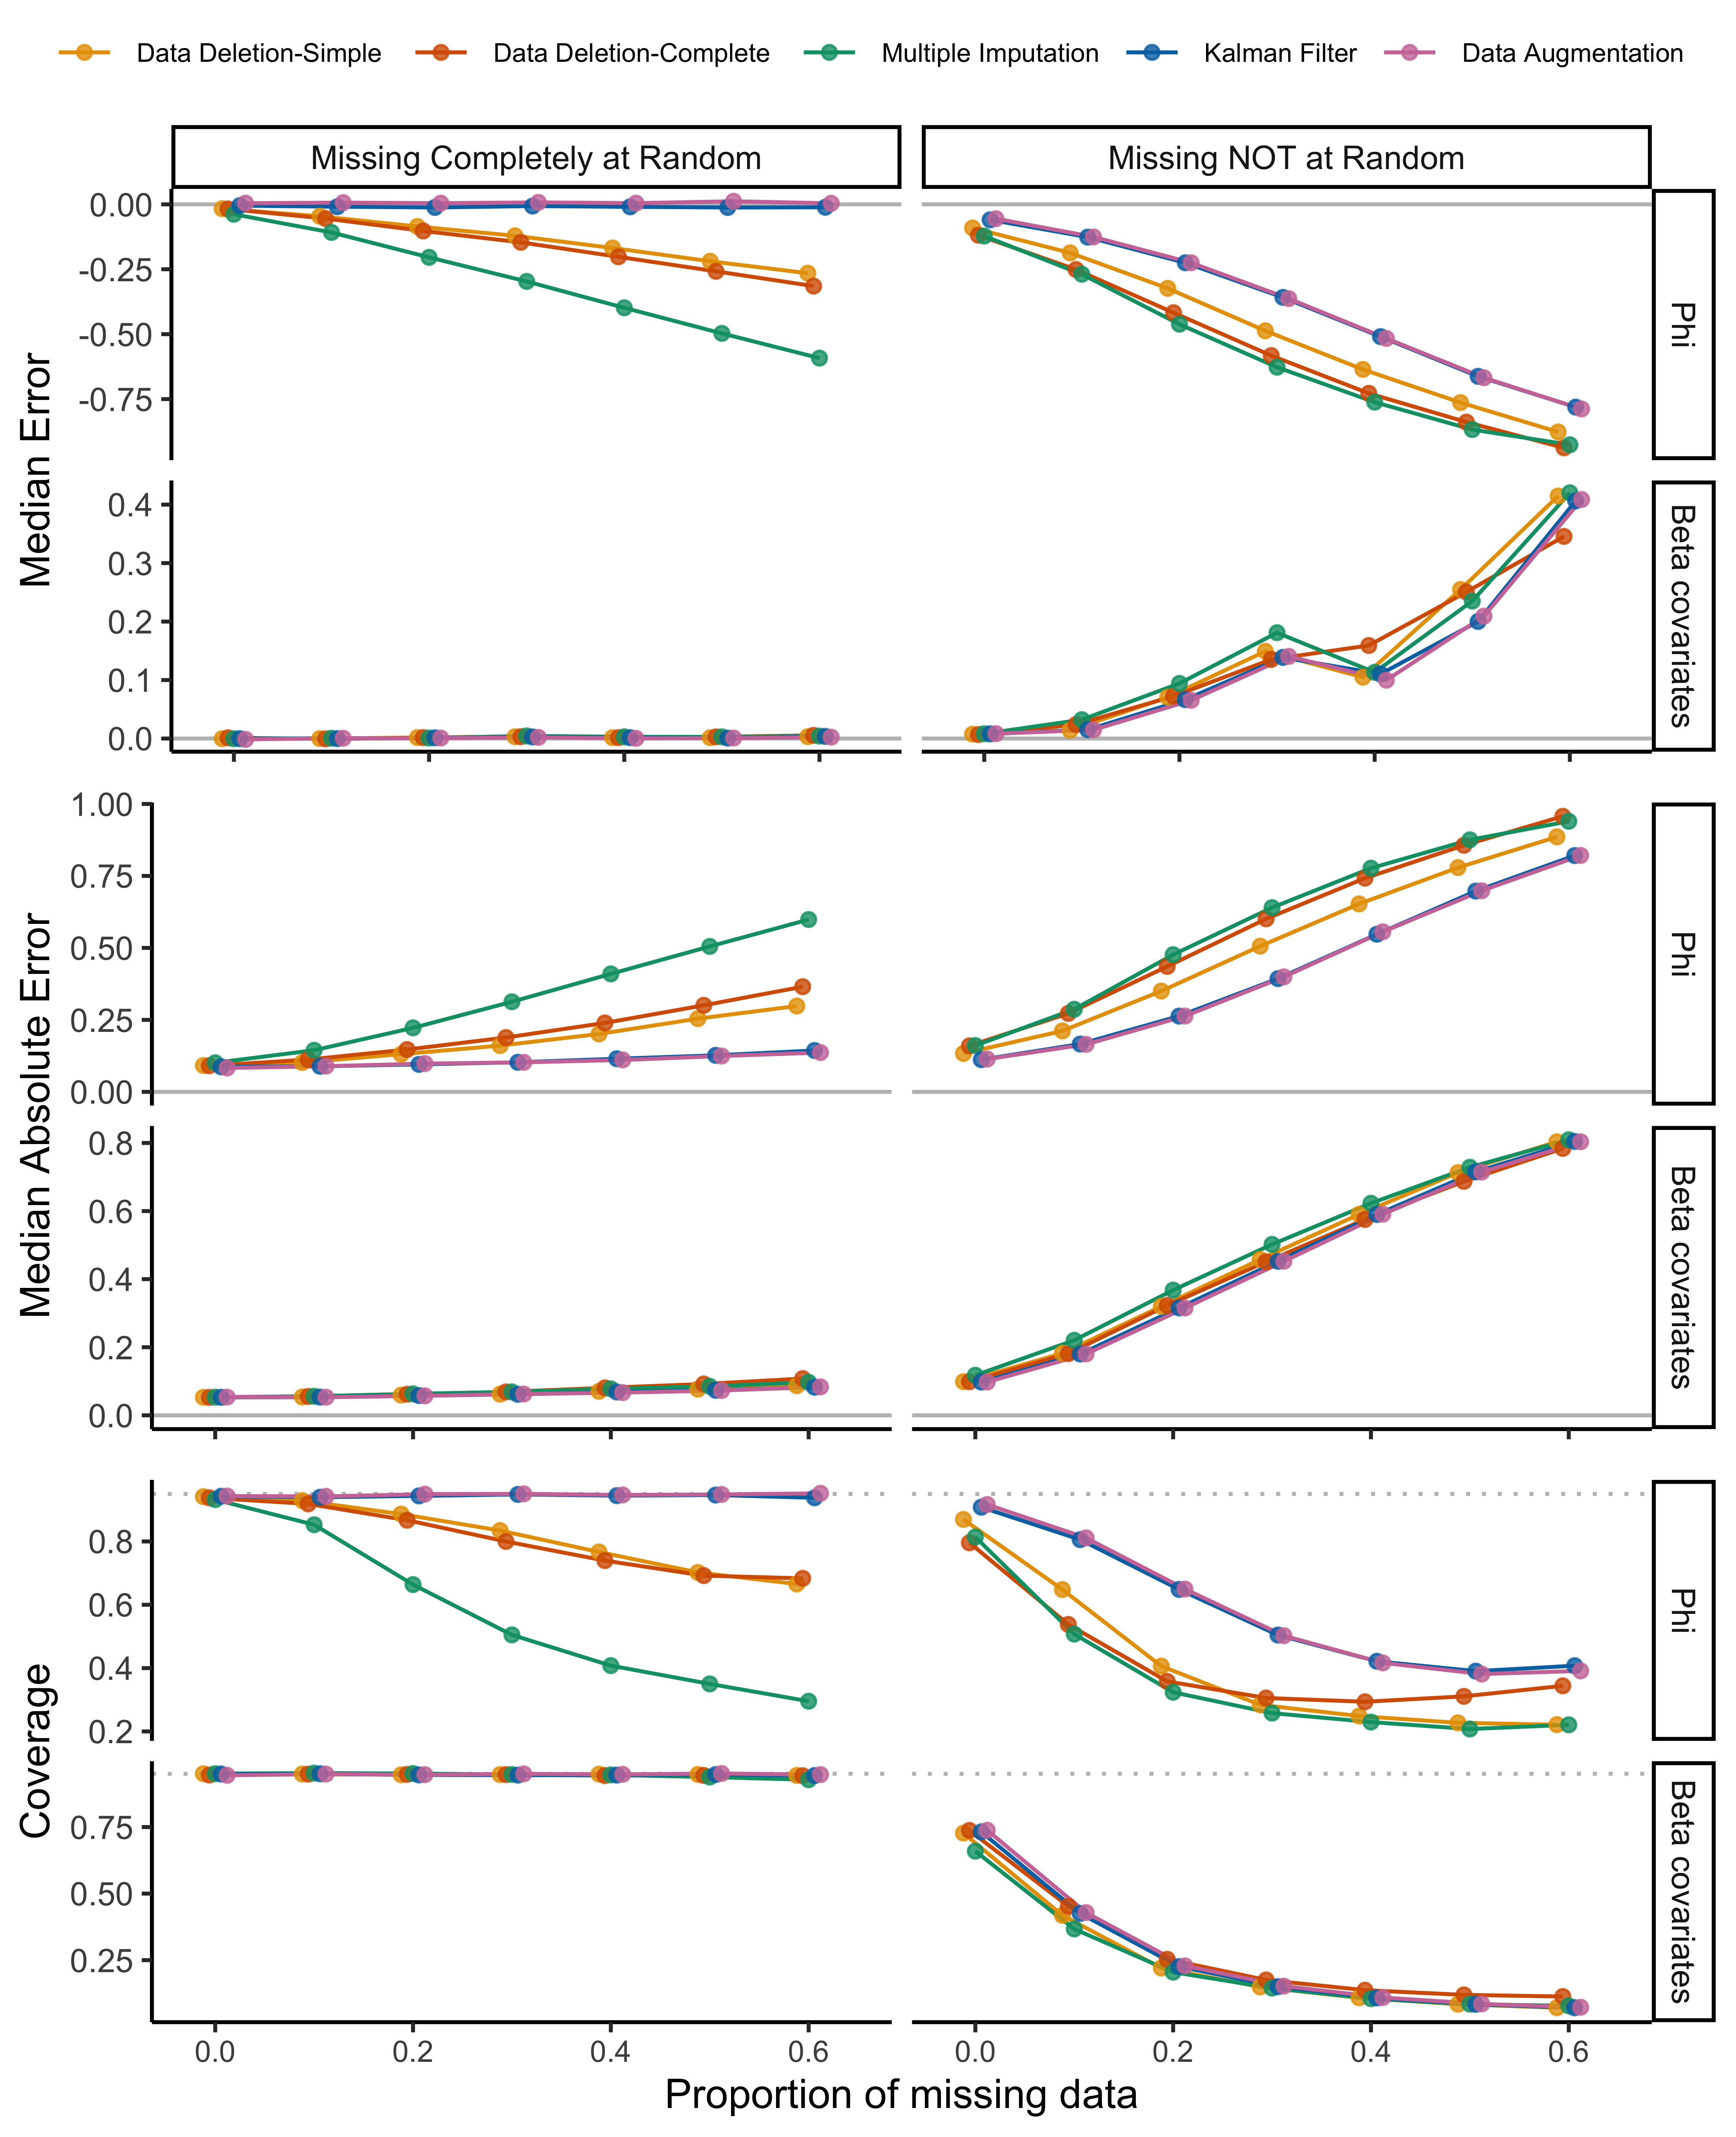
\includegraphics[width = .7\textwidth]{Figures/MockedUpFigures/parameterRecoveryGaussian_MARMNARlong.png}
    \caption{Parameter recovery metrics for Gaussian time series: Here we show the median error of parameter recovery, absolute median error of parameter recovery, and 95\% coverage of parameter estimates, resulting from models fit with five missing data approaches across an increasing proportion of missing data. 
    These models were fit to simulated Gaussian datasets with data missing completely at random (MCAR; left panel) with autocorrelation in missingness between $>$0.3 and $<$ 0.6, and data missing not at random (MNAR; right panel). The coverage panel shows the proportion of model runs where the 95\% confidence interval of a parameter estimate includes the true simulation parameter (dotted line at 0.95). Each point in each panel shows the median value of error or coverage across all models fit to simulations that used the same missing data approach, had the same amount of missing data (within a 10\% bin), approximately the same amount of autocorrelation in missingness, and the same type of missingness.} 

    \label{fig:ParamRec_Gauss}
\end{figure}

%% Figure 4
\begin{figure}
    \noindent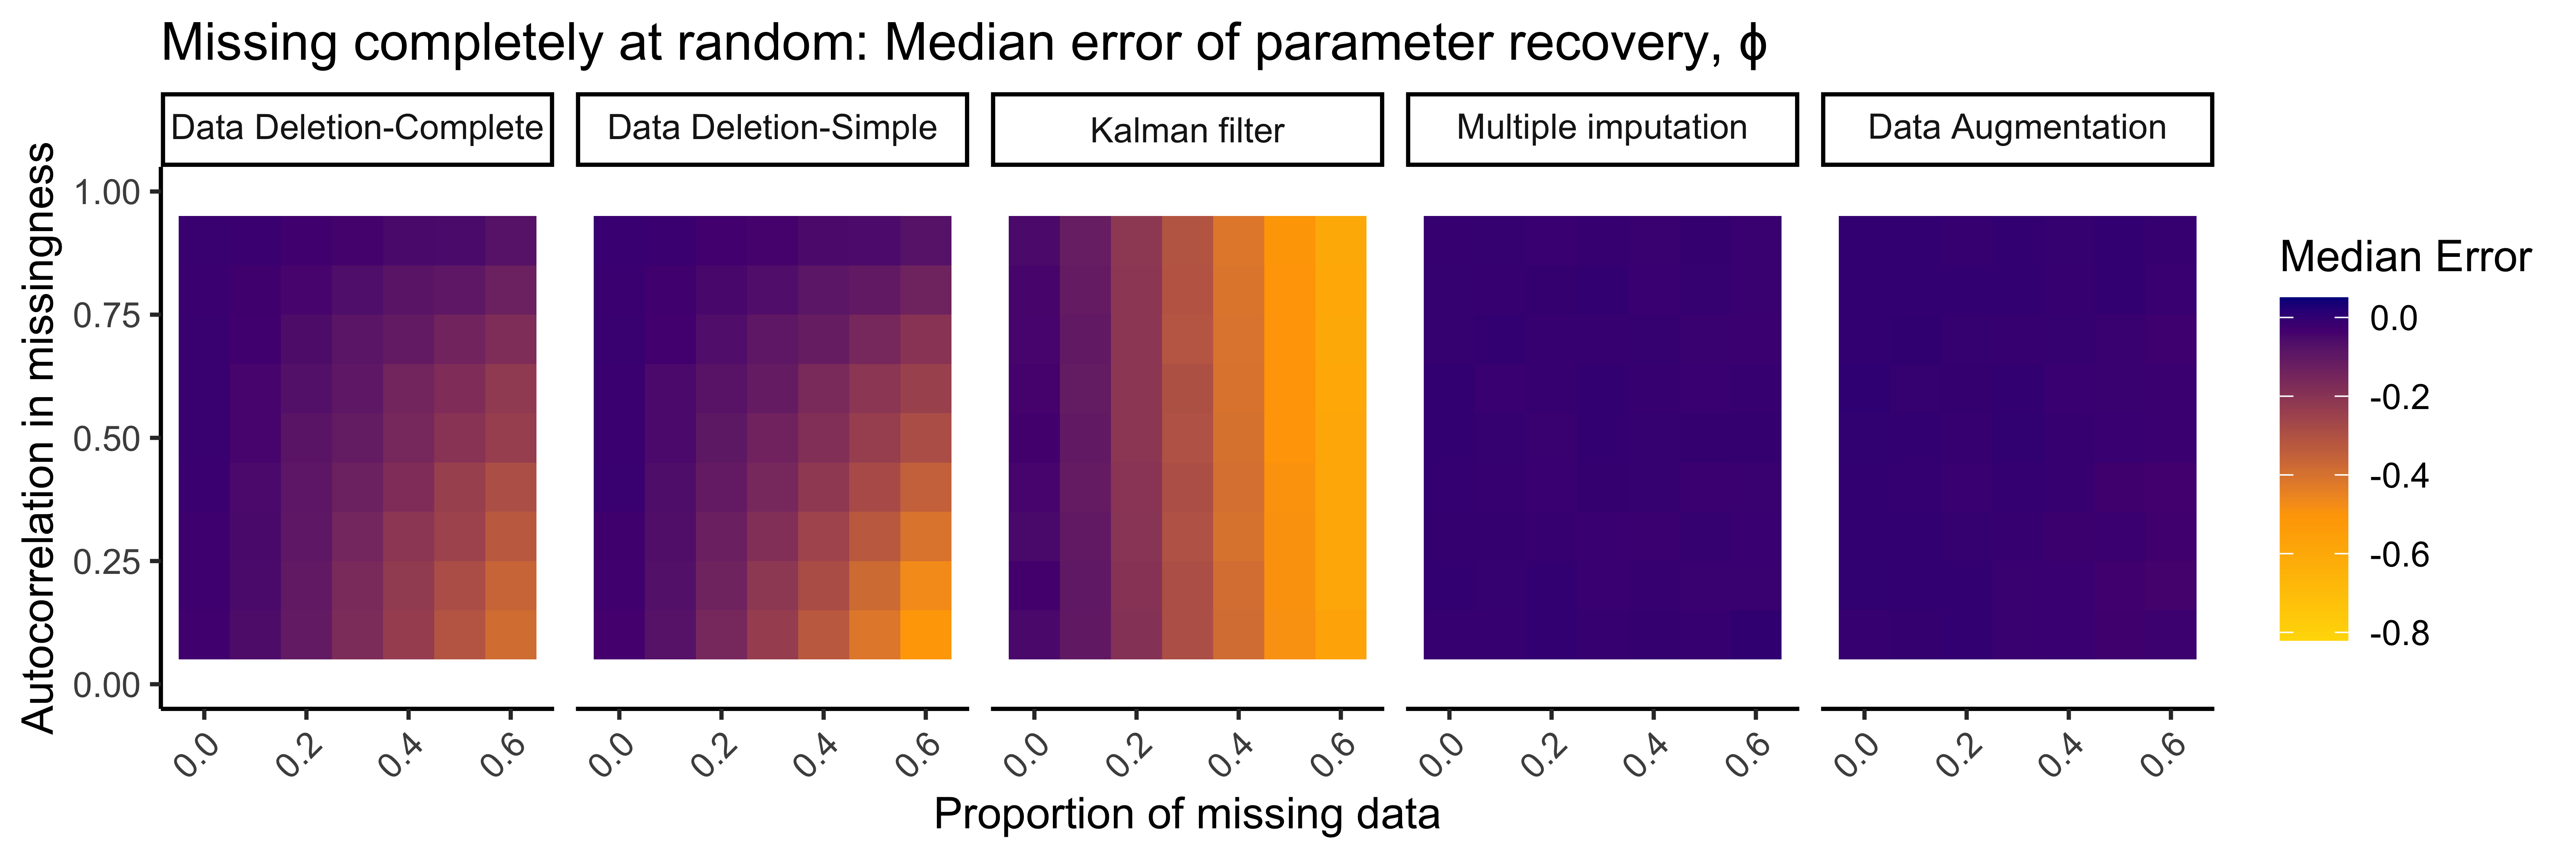
\includegraphics[width = \textwidth]{Figures/MockedUpFigures/heatmap_GaussianMCAR_justPhi.png}

    \caption{Median error of parameter recovery of $\phi$ depending on the proportion of missing data and autocorrelation in missingness for each of five methods missing data approaches, using simulated Gaussian datasets with data missing completely at random (MCAR). Cells in yellow (closer to 0) show that the median of model estimates of $\phi$  were closer to the actual simulation parameter.}

    \label{fig:heatMap_gauss_MAR}
\end{figure}

%% Figure 5
\begin{figure}
    \centering
    \noindent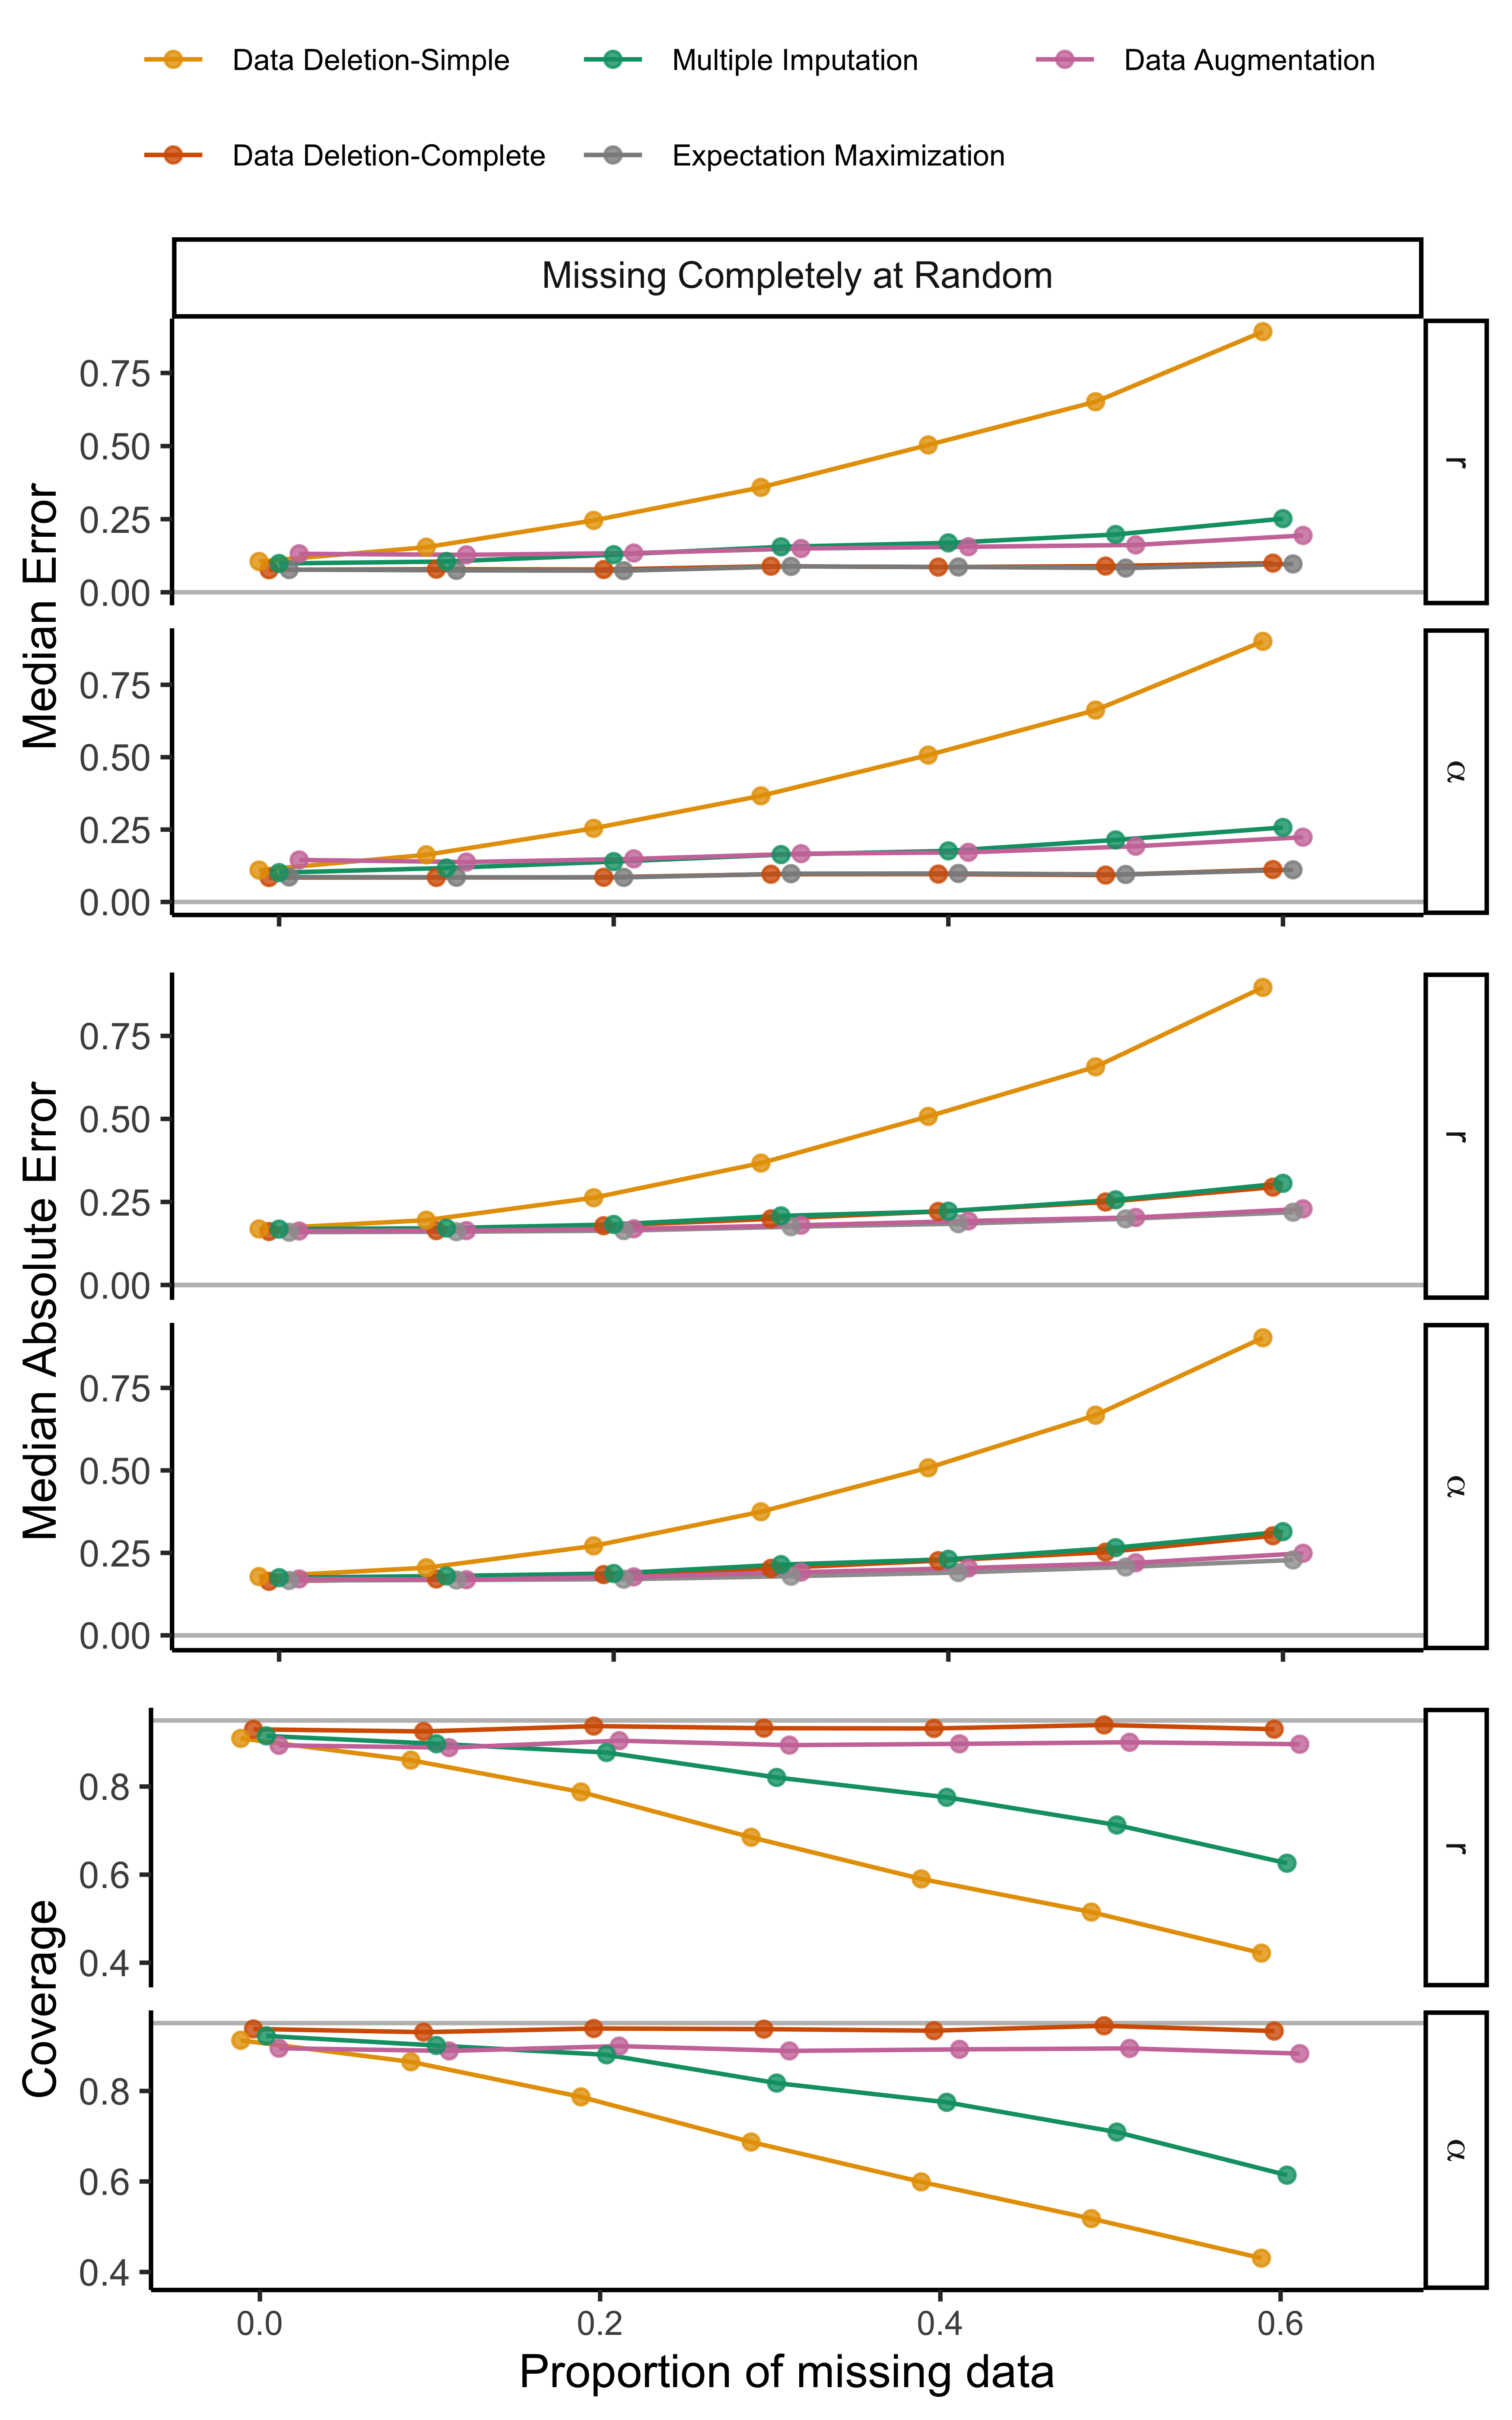
\includegraphics[width = 0.7\textwidth]{Figures/MockedUpFigures/parameterRecoveryPoisson_MCARlong.png}
    \caption{Parameter recovery metrics for Poisson time series: Here we show the median error of parameter recovery, absolute median error of parameter recovery, and 95\% coverage of parameter estimates, resulting from models fit with five missing data approaches across an increasing proportion of missing data. These models were fit to simulated Poisson datasets where data were missing completely at random (MCAR) with autocorrelation in missingness between $>$0.3 and $<$ 0.6. The coverage panel shows the proportion of model runs where the 95\% confidence interval of a parameter estimate includes the true simulation parameter (dotted line at 0.95). Each point in each panel shows the median value of error or coverage across all models fit to simulations that used the same missing data approach, had the same amount of missing data (within a 10\% bin), approximately the same amount of autocorrelation in missingness, and the same type of missingness.}

    \label{fig:ParamRec_Pois}
\end{figure}

%% Figure 6
\begin{figure}
    \centering
    \noindent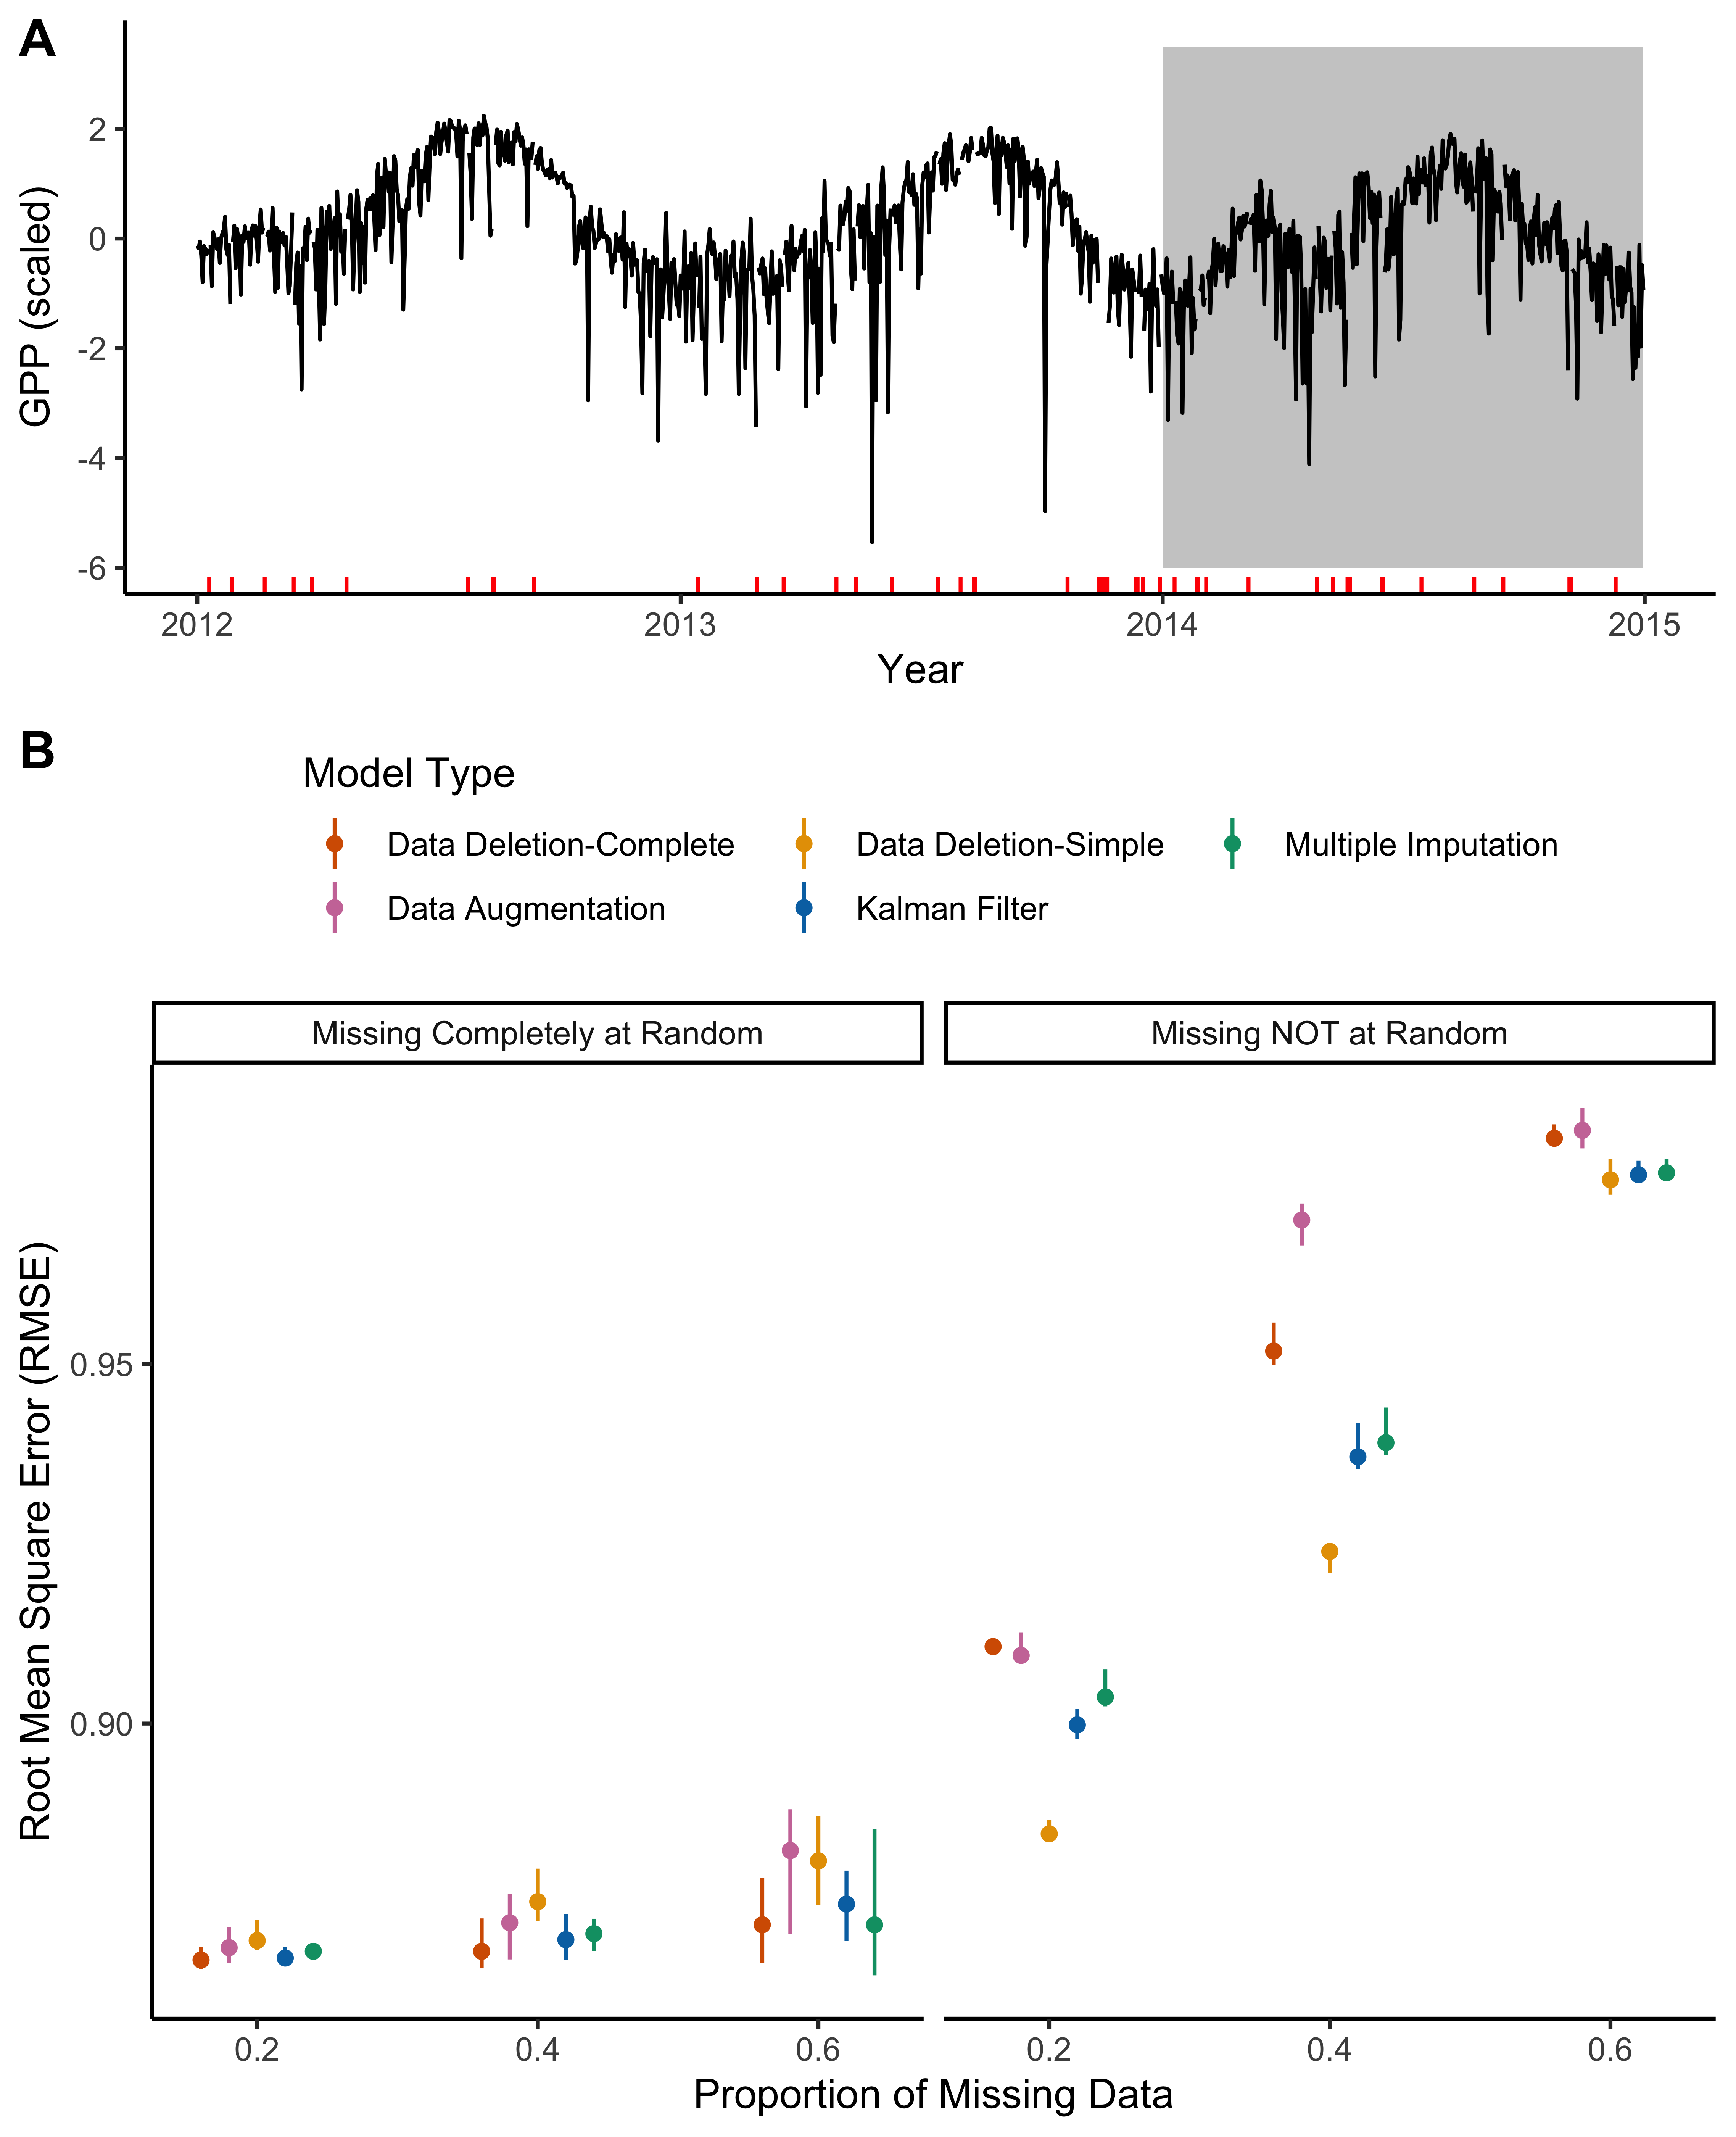
\includegraphics[width = 0.85\textwidth]{Figures/MockedUpFigures/RMSE_FullFigure_NoLineWithErrorBar_gaussian_auSable.png}

    \caption{(A) Daily measurements of scaled gross primary productivity (GPP) from the Au Sable River from 2012 through 2015 (699 days). Red tick marks on the x-axis indicate days when measurements were missing. The gray box indicates the data (347 days) excluded from model fitting, which were then forecast using the resulting model. (B) Root mean square error (RMSE) of forecasts made using a model fit to the Au Sable GPP time series shown in panel A. Each point shows the median RMSE across all forecasts with a given missing data approach (indicated by color), in a given level of proportion of missing data (0.2 $\pm$ 0.05, 0.4 $\pm$ 0.05, 0.6 $\pm$ 0.05), and with a given type of missingness (missing completely at random (MCAR) with autocorrelation of 0.5 $\pm$ 0.05 or missing not at random (MNAR)). Error bars indicate the inter-quartile range.}

    \label{fig:RMSE_Gaus}
\end{figure}

%% Figure 7
\begin{figure}
    \noindent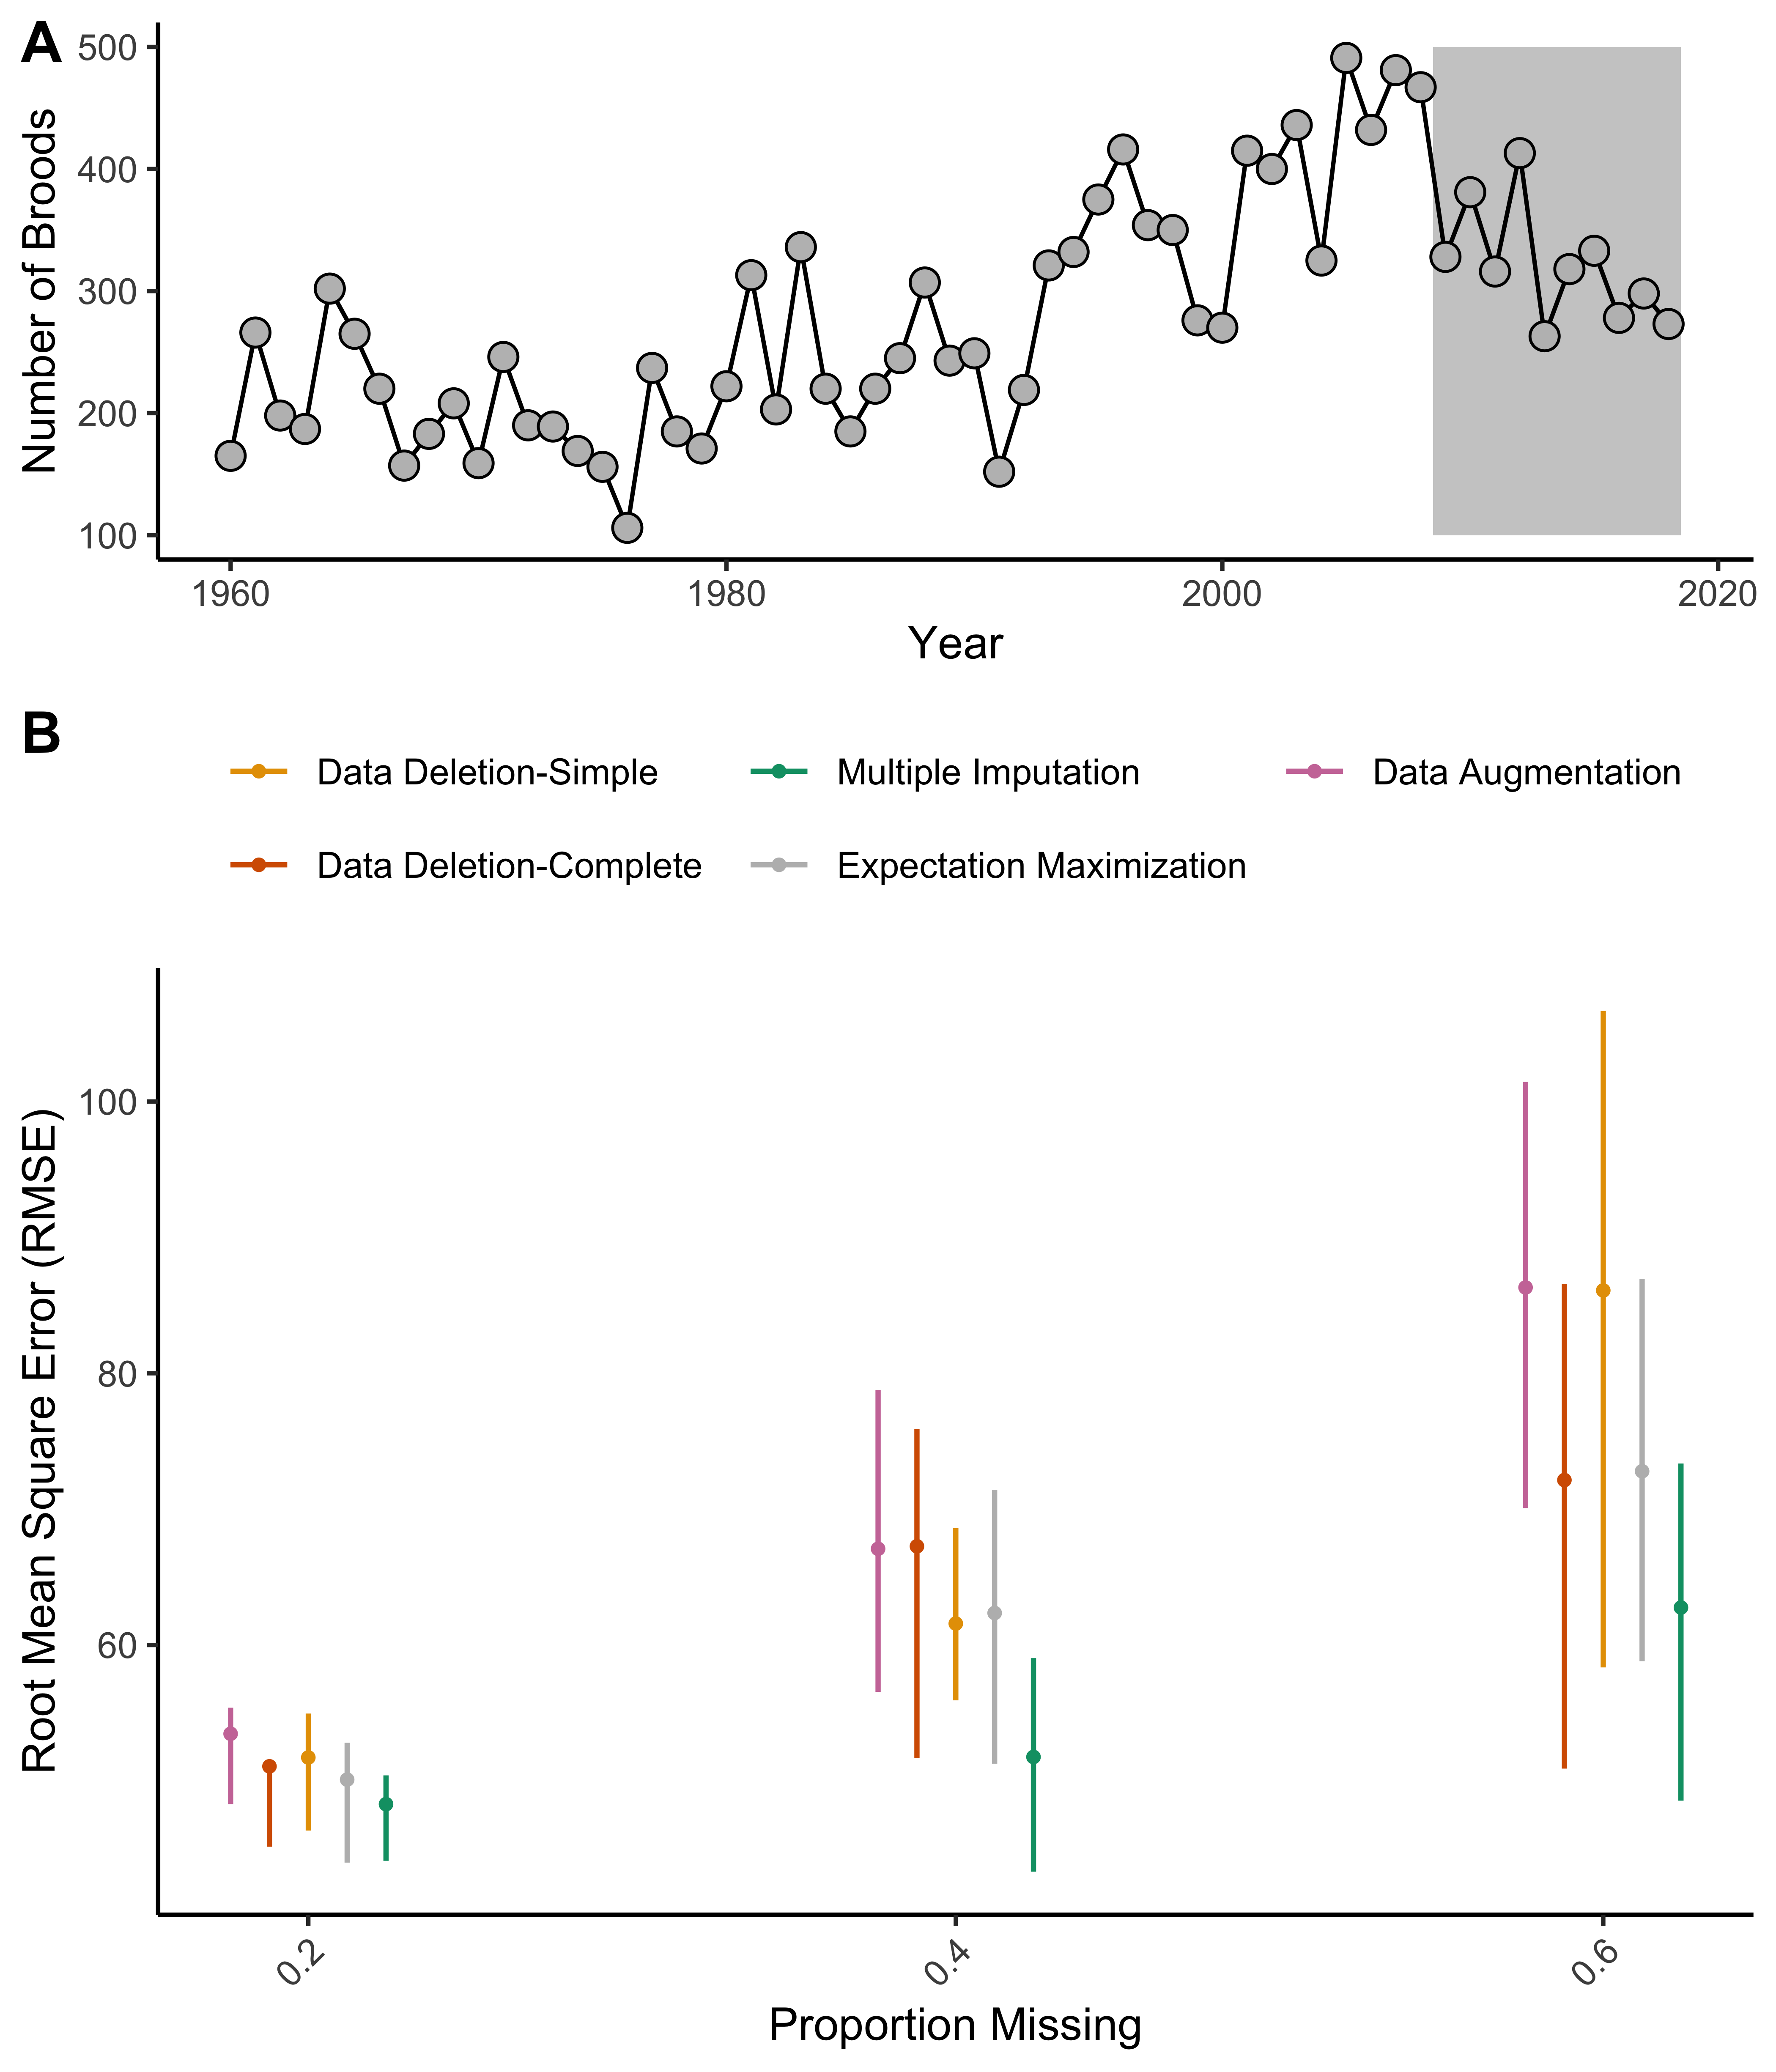
\includegraphics[width = \textwidth]{Figures/MockedUpFigures/RMSE_pois_combined.png}
    \caption{(A) Annual counts of Great Tit (\textit{Parus major}) broods in the Wytham Woods from 1960 – 2018. The gray box indicates the data (10 years) that were excluded from model fitting, which were then forecast using the resulting model. (B) Forecast root mean square error (RMSE) of the Great Tit dataset with an increasing proportion of missing data and missingness approaches. Each point shows the mean RMSE across all forecasts with a given missing data approach (indicated by color), in a given level of proportion of missing data (0.2 $\pm$ 0.05, 0.4 $\pm$ 0.05, 0.6 $\pm$ 0.05) with all bars shown for autocorrelation of 0.5 $\pm$ 0.05. Error bars indicate inter-quartile range}
    \label{fig:RMSE_Poiss}
\end{figure}
\clearpage


\newpage

\bibliographystyle{ecology}
\bibliography{citations}

\newpage

%%\appendix
\documentclass[12pt,english]{article} %12 pt for Ecology %
\usepackage[utf8]{inputenc}

\usepackage{geometry}                		
\geometry{verbose,letterpaper,tmargin=2.54cm,bmargin=2.54cm,lmargin=2.54cm,rmargin=2.54cm}   % 1 inch margins for Ecology   

\usepackage{multirow}
\usepackage{graphicx}		
\graphicspath{ {c:} }
\usepackage{setspace}
\usepackage[version=4]{mhchem}
\doublespace
\usepackage{siunitx}
\usepackage[
  backend=biber,
  style=apa,
  maxcitenames=2,
  natbib=true]{biblatex}
\addbibresource{citations.bib}
\usepackage{amsmath}
\usepackage{bm}
\usepackage{amsfonts}
\usepackage{lineno}
\usepackage{gensymb}
\usepackage[sharp]{easylist}%makes nice outlines.  Use # for symbol
\usepackage{blkarray}
\usepackage{lastpage}
\usepackage{times} % times new roman%
\usepackage{lineno} % add line numbers%

\begin{document}


\noindent\textbf{Journal}: Ecology; \textbf{Article Type}: Statistical Innovations

{\Large \noindent \bf %Approaches for handling missing data in ecological time series
Accounting for missing data in autoregressive models of ecological time series
}

%Journal name
%Manuscript type

\medskip

\noindent Alice E. Stears\textsuperscript{*, 1, 2}, 
Melissa DeSiervo\textsuperscript{*, 3, 2},
Dustin Gannon\textsuperscript{4, 2},
Amy Patterson\textsuperscript{5, 2},
Alice M. Carter\textsuperscript{6,7},
Joanna R. Blaszczak\textsuperscript{8},
Matt Trentman\textsuperscript{9},
Eliza Grames\textsuperscript{10},
Robert O. Hall, Jr\textsuperscript{7},
Joshua P. Jahner\textsuperscript{11, 2},
Saheed O. Jimoh\textsuperscript{2},
Courtenay A. Ray\textsuperscript{2},
Christa L. Torrens\textsuperscript{7},
Lauren Shoemaker$^{\circ}$\textsuperscript{2},
Christopher Weiss-Lehman$^{\circ}$\textsuperscript{2}

\noindent\noindent \textbf{Author affiliations}

\noindent\textsuperscript{1} Center for Adaptable Western Landscapes, Northern Arizona University, Flagstaff, AZ

\noindent\textsuperscript{2} Botany Department, University of Wyoming, Laramie, WY

\noindent\textsuperscript{3} Biology Department, Union College, Schenectady, NY

\noindent\textsuperscript{4} Department of Forest Ecosystems and Society, Oregon State University, Corvallis, OR 

\noindent\textsuperscript{5} Department of Biology, University of Maryland, College Park, MD

\noindent\textsuperscript{6} Department of Mathematics and Statistics, Utah State University, Logan, UT

\noindent\textsuperscript{7} Flathead Lake Biological Station, University of Montana, Polson, MT

\noindent\textsuperscript{8} Department of Natural Resources and Environmental Sciences, University of Nevada, Reno, Reno, NV

\noindent\textsuperscript{9} O’Connor Center for the Rocky Mountain West, University of Montana, Missoula, MT

\noindent\textsuperscript{10} Biological Sciences, Binghamton University, State University of New York, Binghamton, NY

\noindent\textsuperscript{11} Department of Biology, New Mexico Institute of Mining and Technology, Socorro, NM

\noindent\textsuperscript{*} Denotes equal contribution as lead author

\noindent{$^{\circ}$} Denotes equal contribution as primary investigator

\noindent \textbf{Corresponding author}: Alice Stears, alice.e.stears@gmail.com 


\section*{Appendix S1}


\subsection*{Introducing Missingness}

We created MCAR datasets with varying proportions of missing data and degrees of autocorrelation in missingness (Fig. \ref{fig:missingtypes} B--E) by viewing a time series as a Markov-modulated Bernoulli process where the variable could have two states: missing or not missing \citep{Gharib2014, Edwards1960}. The probability that an observation in a time series at time $t+1$ was missing depended on both the specified proportion of non-missing values in the entire time series ($p$) and the specified degree of autocorrelation in missingness ($\omega$). In a time series $X_1, X_2, ..., X_n$, the transition matrix that describes the probability of an observation at $X_{t+1}$ being missing, based on whether the observation at $X_t$ was missing is defined as: 


\begin{equation}
\begin{blockarray}{rcccc}
\text{} & \BAmulticolumn{4}{c}{X_{t+1}}\\
X_t & \text{Present} & \text{Missing}  \\
\begin{block}{r(cccc)}
\text{Present} & 1-(1-\omega)p & (1-\omega)p \\
\text{Missing} & (1-\omega)(1-p) & \omega + (1-\omega)p  \\
[1ex]
\end{block}
\end{blockarray}
\end{equation}


We created MNAR datasets with various proportions of msising data by first calculating the mean and standard deviation of the time series with no missing data, then using these point estimates as the mean and standard deviation of a normal distribution. We then identified the quantiles of that normal distribution above and below which the density of the normal distribution corresponded to the desired proportion of missingness. We replaced any values above and below those quantiles with an NA.

\subsection*{Missing Data Approaches} 
\textbf{Simple and Complete Data Deletion}: The ``simple data deletion" approach involves removing missing values from a time series, compressing the dataset, and running the model as if the time intervals between observations were all equal (Fig. 1 A). This method violates the assumption of equal temporal spacing between observations, an assumption implicit in most time series models. We include it here as a reference because it is simple and commonly used in published studies. We also include ``complete case data deletion," which maintains equal spacing between observations by removing a missing value itself as well as the subsequent observation(s) that is predicted by the missing value (Fig. 1 A). However, those observations after a missing value are retained as predictors of the subsequent observation(s). 

\textbf{Multiple Imputation}: Multiple imputation (MI) is an approach that systematically fills in missing observations with imputed values, and creates several versions of complete data sets that can be used to estimate uncertainty around each imputed value (Fig. 1 B). MI is commonly used in ecology, with multiple studies evaluating methods and approaches to conduct MI for functional traits \citep{taugourdeau_filling_2014,johnson_handling_2021,penone_imputation_2014}, population biology \citep{onkelinx_working_2017}, time series \citep{hui_gap-filling_2004}, and meta-analyses \citep{ellington_using_2015}. Multiple Imputation’s (MI) effectiveness can depend on the number of imputed datasets (\textit{m}). It is often assumed that \textit{m}=5 is a minimum value \citep{honaker_what_2010}; however, researchers have used \textit{m}=200 when comparing methods in the ecological sciences \citep{onkelinx_working_2017}. In general, larger values of \textit{m} result in more accurate estimates of both parameter values and uncertainty. However, increasing \textit{m} results in a trade-off between accuracy and computation time; this can be particularly problematic for data-rich (e.g., long time series) or complex (e.g., hierarchical) models. 
After imputing the \textit{m} data sets, the analyses of interest are confronted with each data set, and the estimated parameters from the \textit{m} analyses are averaged using Rubin rules of averaging to get the parameter(s), and associated uncertainty, from which inference can be made. We implemented multiple imputation with the Amelia II package in R \citep{honaker2011}, which uses an expectation maximization algorithm (see below) in combination with a bootstrapping technique for deciding what values to impute. We used $m=5$ in order to provide decent estimates without excessive run times.

For both the simulated and empirical population count time series, since we did not have any covariates, the only variables used for imputation were the population size at time \textit{t} and population size at time \textit{t-1}. For time series with chunks of missing data, the Amelia multiple imputation function had to be run iteratively, with missing values filled in from the edges of the missing chunks. In addition, while the recommended settings for dealing with time series data using the Amelia package include incorporating preceding and proceeding time points by specifying the ``lags" and ``leads" options \citep{honaker2011}, it was not possible to use the lags option, since the current population was already using the population at the previous point as its only predictor for imputation. Instead, we included only the leads option, which still resulted in occasional failure of the method at extremely high levels ($>70\%$) of missing data due to excessive collinearity between the preceding and proceeding time points. The lack of error handling for extremely collinear variables is an unfortunate issue for this method when using data sets without covariates, or data sets with highly collinear covariates.  

For both the simulated and empirical Gaussian series, implementing multiple imputation was more straightforward since an observation at time \textit{t} was informed by two covariates in addition to the observation at the time \textit{t-1}. In this case, we were able to use both the ``lags" and ``leads" options in \texttt{amelia}. 

Following execution of MI using Amelia II, we fit statistical models to time series following the methods described in \textbf{Main Text: Comparing missing data approaches}.

\textbf{Kalman Filter}: The Kalman Filter (KF) was developed to estimate the state of a dynamic system that is observed with error but can be used to derive the likelihood function of a time series with missing observations (Fig. 1 C). To illustrate the approach, assume a state-space model

\begin{equation}
    \begin{aligned}
        X_t &= \phi X_{t-1} + \epsilon_t \\Y_t &= X_t + e_t
    \end{aligned}
\end{equation}
where $X_t$ is the true ``state" of the system at time $t$, $Y_t$ is the observed value at time $t$, and $\epsilon_t \sim \mathcal{N}(0, \sigma^2)$ and $e_t \sim \mathcal{N}(0, \tau^2)$ are IID white noise error terms for the process and observation error, respectively. The Kalman Filter is primarily focused on estimating the unobserved state of the system, $X_t$, and can be conceptualized as a two-step procedure in which, given an initial state $X_0$, we can forecast the next state $X_1$. Then, following data collection at the next time point, $y_1$, we update the forecast using Bayes' theorem. Specifically, the forecast distribution for $X_1$ is
\begin{equation}
    p(x_1) = \int p(x_1 | x_0)p(x_0)dx_0
\end{equation}
where $p(\cdot)$ denotes the probability density function. Assuming IID Gaussian errors, $p(x_1)$ is normal with mean ${\tilde x}_1 = \phi x_0$ and variance $v_1 = \phi^2 \frac{\sigma^2}{1 - \phi^2} + \sigma^2$. Given the observed value $y_1$, we update the estimate of $X_1$ using Bayes theorem
\begin{equation}
    \begin{aligned}
        p(x_1 | y_1) &\propto p(y_1 | x_1) p(x_1)
        &= \mathcal{N}\Bigl(\tilde x_1 + K_1(y_1 - \tilde x_1),\ (1 - K_1)v_1 \Bigr)
    \end{aligned} 
\end{equation}
where $K_1 = v_1 / (v_1 + \tau^2)$ is the \textit{Kalman gain} and creates a weighted average of the forecast and observation. %If the observation error is large, the forecast is favored as an estimate of $X_t$, whereas if the process noise is large relative to the observation error, the estimate of $X_t$ tends towards the observed value $y_t$.
For our focus on missing data, we assume the process is observed without error such that $Y_t = X_t$ and $\tau^2 = 0$. Without observation error, the Kalman gain $K_t = 1$ for all $t$ since $\tau^2 = 0$, and $p(x_1 | y_1) = \mathcal{N}(y_t, 0)$. Thus, the update step gives complete information about $X_t$, and the likelihood function can be defined based on the data $y_1,...,y_n$. However, if data are missing, the update step cannot occur. So, in the case of missing data without observation error, the Kalman Filter alternates between pure forecast steps when data are missing and pure ``update" steps when data and the state of the system are completely observed, but the forecast steps yield a method for computing the likelihood function recursively without needing to know the states of $X_t$ in which we were unable to observe the process and therefore have no associated $y_t$.

The Kalman filter assumes a Gaussian error distribution, so we only used this method with the simulated and empirical real-valued time series. We implemented KF missing data approach at the same time as the model fitting process, where we fit an AR(1) model with two covariates using the \texttt{arima} function from the \texttt{stats} package in R \citep{r_2021} (KF is the default algorithm used to handle missing values in this R function). 


\textbf{Expectation Maximization}: The expectation maximization (EM) algorithm is an iterative algorithm that is conceptually similar to KF, and recursively computes the likelihood of a time series with missing data (Fig. 1 D). Given an initial guess for the parameter vector we wish to estimate, ${\bm \theta}_0$, the first step (Expectation step) proceeds to ``fill in" the missing observations with their expectation given the observed data and the initial parameter vector ${\bm \theta}_0$ %. For example, if $Y_t$ were missing, we impute $Y_t$ with $\mathbb{E}(Y_t | y_{t-1}, {\bm \theta}_0)$
, which is equivalent to the forecast step of the Kalman filter conditioned on ${\bm \theta}_0$. In the second step (maximization step), we compute the maximum likelihood estimate of ${\bm \theta}$ using the filled-in time series as data to give an updated estimate $\hat {\bm \theta}_1$. We then iterate this process, updating the forecasts of the missing data using their expectations conditional on $\hat {\bm \theta}_1$, then maximizing the likelihood with respect to $\bm \theta$ using the time series filled-in with the updated forecasts. This process is iterated until the difference between successive estimates is acceptably small, indicating convergence (that is, $||\hat {\bm \theta}_i - \hat {\bm \theta}_{i-1}||_1 < \delta$ for some small $\delta > 0$).

Given its similarity to KF, we only used this missing data approach for the simulated and empirical times series of counts. We constructed an approximate EM algorithm to estimate the parameters of the Ricker model in which missing data were rounded to the nearest integer value during the expectation step such that the likelihood was well-defined for the filled-in series. As such, the missing data were dealt with at the same time as the model fitting process. We used the \texttt{optim} function from the \texttt{stats} package in \texttt{R} for the maximization step \citep{r_2021}. %In Figure S2%\ref{fig:EM-bias-checks}
%, we show that the estimates are asymptotically unbiased. 
Note that the algorithms required to estimate standard error of parameter estimates generated from EM are notoriously unstable and difficult to implement in R, so the results of models we fit using this missing data approach do not include standard error estimates. 

\textbf{Data Augmentation}: Data augmentation (DA) provides a model-based framework for estimating missing observations as well as the parameters of interest, but comes with the added benefit of standard errors for the estimates of all the unknown quantities by treating the missing observations as additional parameters to be estimated (Fig. 1 D). We fit the Gaussian AR(1) models with DA and Stan \citep{carpenter_stan_2017} by using the rstan \citep{rstan_package} and brms \citep{burkner2017brms} packages in R \citep{r_2021}. Data augmentation for the population model is not possible with Stan, however, due to the requirement of continuous parameter space for the Hamiltonian Monte Carlo (HMC) methods Stan uses to sample the posterior distribution (at least not without marginalizing out the discrete parameters, which proved intractable). Treating missing integer data as parameters was therefore not possible with Stan, and partially-known parameter vectors are not supported in JAGS. We therefore designed a Gibbs sampler with Metropolis updates for the log growth factor ($r$) and intra-specific competition coefficient ($\alpha$), and Gibbs sampling of any missing observations, $N_{t}^{(0)}$, conditional on $(r, \alpha, {\bf N}_{t-})$, where ${\bf N}_{t-}$ is the vector of abundances (both observed and unobserved) up to but not including time $t$. We used weakly informative Gaussian priors for $r$ and $\ln(\alpha)$ and fit the models using custom functions written in R. 


\printbibliography

%\bibliographystyle{ecology}
%\bibliography{citations}


\renewcommand{\figurename}{Figure}
\renewcommand{\thefigure}{S\arabic{figure}}
\begin{figure}
     \noindent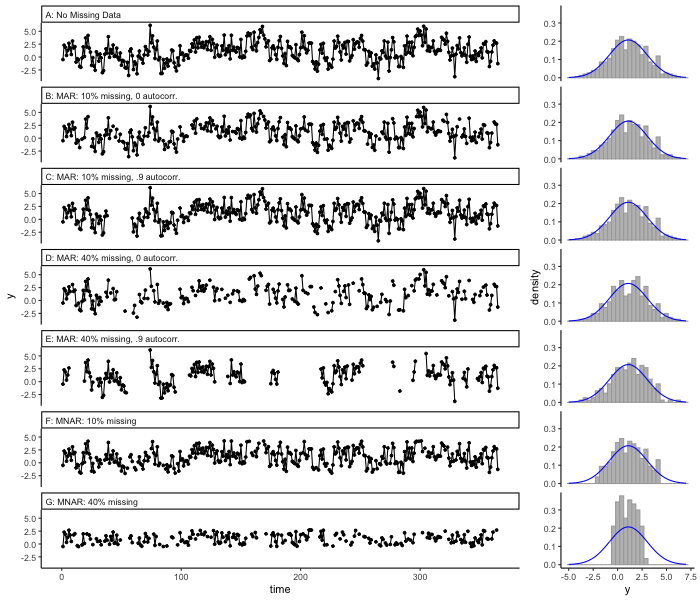
\includegraphics[width = 0.85\textwidth]{Figures/CompareMissingnessTypes_fig.png}
     \caption{An example time series demonstrating different types and amounts of missing data. The left column shows the same time series with different amounts and types of missingness and right column shows the distribution of data points in each resultant time series. A. Complete time series with no missing data. Rows B through E show the time series with 10\% (B and C) or 40\% (D and E) of data missing completely at random (MCAR), with either low autocorrelation in missing data (B and D) or high autocorrelation (C and E). Rows F and G show the time series with data missing not at random (MNAR) for 10\% missing data (F) and 40\% missing data (G).}
     \label{fig:missingtypes}
 \end{figure}

 \begin{figure}
     \noindent\includegraphics[width = 0.85\textwidth]{Figures/MockedUpFigures/heatmap_GaussianMCAR_all.png}
     \caption{Median error of parameter recovery, median absolute error, and model coverage of $\phi$ and $\beta$, depending on the proportion of missing data and autocorrelation in missingness for each of five missing data approaches, using simulated, real-valued datasets with data missing completely at random (MCAR).}
     \label{fig:GaussianMCARheatmapALL}
 \end{figure}

  \begin{figure}
         \noindent\includegraphics[width = 0.85\textwidth]{Figures/MockedUpFigures/heatmap_PoissonMCAR_all.png}
     \caption{Median error of parameter recovery, median absolute error, and model coverage of $\alpha$ and $r$, depending on the proportion of missing data and autocorrelation in missingness for each of five missing data approaches, using simulated time series of counts with data missing completely at random (MCAR). Note that coverage is not shown for the Expectation Maximization approach, since most implementations of this method do not include estimates of standard error.}
     \label{fig:PoissonMCARheatmapALL}
 \end{figure}
 
%\subsection{Bias due to endogeneity}

%It is well known that the ordinary least squares estimator (OLS) of the autoregressive coefficients in an AR($p$) model is biased. To see this, consider a simple AR(1) model with mean zero and variance of the innovations $\sigma^2$. The model can be written as
%$$
%y_t = \phi y_{t-1} + \epsilon_t
%$$
%where $\epsilon_0, ..., \epsilon_n \overset{iid}{\sim} \mathcal{N}(0, \sigma^2)$ and $\phi$ is the autoregressive coefficient. The OLS estimator of $\phi$, $\hat{\phi}$ is obtained by regressing observations $y_1,...,y_n$ against $y_0,...,y_{n-1}$. Thus, the OLS estimator can be written as
%\begin{equation*}
%    \begin{aligned}
%        \hat{\phi} &= \frac{\sum_{t=1}^n y_t y_{t-1}}{\sum_{t=1}^n y_{t-1}^2}\\
%        &= \frac{\sum_{t=1}^n (\phi y_{t-1} + \epsilon_t) y_{t-1}}{\sum_{t=1}^n y_{t-1}^2}\\
%        &= \frac{\sum_{t=1}^n (\phi y_{t-1}^2 + \epsilon_t y_{t-1})}{\sum_{t=1}^n y_{t-1}^2} \\
%        &= \phi \frac{\sum_{t=1}^n y_{t-1}^2}{\sum_{t=1}^n y_{t-1}^2} + \sum_{t=1}^n \frac{y_{t-1}}{\sum_{t=1}^n y_{t-1}^2} \epsilon_t\\
%        &= \phi + \sum_{t=1}^n \frac{y_{t-1}}{\sum_{t=1}^n y_{t-1}^2} \epsilon_t.
%    \end{aligned}
%\end{equation*}
%Taking the expectation,
%\begin{equation*}
%    \mathbb{E}(\hat \phi) = \phi + \mathbb{E}\left(\sum_{t=1}^n \frac{y_{t-1}}{\sum_{t=1}^n y_{t-1}^2} \epsilon_t \right)
%\end{equation*}
%we see that, because the sum in the denominator of the second term in the expectation, $\sum_{t=1}^n y_{t-1}^2$, is not independent of $\epsilon_t$ (if $\epsilon_t$ is large and positive, the sum in the denominator will also increase), the ``covariate" we use is \textit{endogenous}, meaning it is not independent of the errors. The negative correlation between $\epsilon_t$ and the reciprocal of sum $\sum_{t=1}^n y_{t-1}^2$ results in a downward-biased estimator of $\phi$ (i.e, closer to zero). 




\newpage


\end{document}

%%%%%%%%%%%%%%%%%%%%%%%%%%%%%%%
\end{document}
%%%%%%%%%%%%%%%%%%%%%%%%%%%%%%%
